%\documentclass[compress]{beamer}
\documentclass[handout]{beamer}




%%%%%%%%%%%%%%%%%%%%%%%%%%%
% LaTeX package inclusion %
%%%%%%%%%%%%%%%%%%%%%%%%%%%
\usepackage{times}
\usepackage{units}
\usepackage{mathrsfs}
\usepackage{diss} % defines \bv and some other stuff
\usepackage{subfigure}
\usepackage{multirow}
\usepackage{amsmath}
\usepackage{amssymb}
%\usepackage{algorithm}
%\usepackage{algorithmic}
\usepackage{hyperref}
\usepackage{listings}
\usepackage{movie15}
\usepackage{stmaryrd} % \llbracket
\usepackage{cancel} % \cancel
\graphicspath{{figs/}}



\usefonttheme[
  onlymath
]{serif} %onlymath option doesn't look too bad, eqns are more readable this way.

\definecolor{DarkGreen}{rgb}{0.13,0.55,0.13}
\definecolor{DarkRed}{rgb}{0.55,0.13,0.13}
\definecolor{mygray}{rgb}{0.5,0.5,0.5}
\definecolor{mymauve}{rgb}{0.58,0,0.82}
\setcounter{tocdepth}{1}


\usetheme{pecostalk}

\definecolor{nasablue}{RGB}{0,96,169}
\definecolor{nasared}{RGB}{239,61,66}
\definecolor{orionblue}{RGB}{15,16,64}

%\usecolortheme{orchid} % white on dark block titles.  use w/ whale.
%\usecolortheme{whale} % darkest top titles, usually used by CFDLab presenters
\setbeamertemplate{itemize items}[circle]% Force any theme (eg Antibes) to use circle bullets
%\useinnertheme[shadow]{rounded} % Causes itemize blocks to have rounded corners & drop shadows
%\logo{
\includegraphics[width=.5in]{common/rawfigs/word3}}
%\setbeamercolor{title}{fg=red!80!black,bg=red!20!white} %pink title!

\title[\texttt{libMesh} FE Library]{\texttt{libMesh} Finite Element Library:
Design, Use, and Abuse}
\author[R.~H.~Stogner]{Roy H. Stogner}
\institute[INL]{Idaho National Laboratory}
\date{February 27, 2025}


\newcommand{\R}{\mathscr{R}}
\newcommand{\libMesh}{\texttt{libMesh}}
\newcommand{\PETSc}{\texttt{PETSc}}
\newcommand{\cpp}{\texttt{C++}}
\newcommand{\emphcolor}[1]{\textcolor{nasablue}{#1}}
\newcommand{\royslide}[2]{\begin{frame} \frametitle{#1} #2 \end{frame}}
\newcommand{\royitemizebegin}[1]{\begin{block}{#1} \begin{itemize}}
\newcommand{\royitemizeend}{\end{itemize} \end{block}}
\newcommand{\commentout}[1]{}

\newcommand{\V}[1]{\bv{#1}}
\newcommand{\M}[1]{\bv{#1}}
\newcommand{\orderof}[1]{\ensuremath{ {\cal O}\left(#1\right)}}
\newcommand{\Reals}{\mathbb{R}}
\newcommand{\abs}[1]{\ensuremath{ \left|#1\right|}}
\newcommand{\norm}[1]{\ensuremath{ \left|\left|#1\right|\right|}}

\newcommand{\Qoi}{{\ensuremath{Q}}}
\newcommand{\qoi}{{\ensuremath{q}}}
\newcommand{\Res}{{\ensuremath{\mathcal R}}}
\newcommand{\params}{{\ensuremath{\bv{\xi}}}}
\newcommand{\Unknowns}{{\ensuremath{\bf{U}}}}
\newcommand{\unknown}{{\ensuremath{\bv{u}}}}
\newcommand{\Testfuncs}{{\ensuremath{\bf{V}}}}
\newcommand{\primalsol}{{\ensuremath{\bv{\tilde{u}}}}}
\newcommand{\primalsolh}{{\ensuremath{\bv{\tilde{u}^h}}}}
\newcommand{\adjointsol}{{\ensuremath{\bv{\tilde{z}}}}}
\newcommand{\adjointsolh}{{\ensuremath{\bv{\tilde{z}^h}}}}
\newcommand{\adjointsolH}{{\ensuremath{\bv{\tilde{z}^H}}}}
\newcommand{\Liftfunc}{{\ensuremath{\Psi}}}
\newcommand{\elem}{\ensuremath{E}}




\AtBeginSection[]
{
   \begin{frame}
       \frametitle{Outline}
       \tableofcontents[currentsection]
   \end{frame}
}


\begin{document}

\lstset{
  language=C++,
  basicstyle=\scriptsize\ttfamily,
  frame=none,
  commentstyle=\color{nasared},
  keywordstyle=\color{nasablue},   % keyword style
  numbers=none,                    % where to put the line-numbers; possible values are (none, left, right)
  numbersep=3pt,                   % how far the line-numbers are from the code
  numberstyle=\tiny\color{mygray}, % the style that is used for the line-numbers
  rulecolor=\color{black},         % if not set, the frame-color may be changed on line-breaks within not-black text
  showspaces=false,                % show spaces everywhere adding particular underscores; it overrides 'showstringspaces'
  showstringspaces=false,          % underline spaces within strings only
  showtabs=false,                  % show tabs within strings adding particular underscores
  stepnumber=2,                    % the step between two line-numbers. If it's 1, each line will be numbered
  stringstyle=\color{mymauve}      % string literal style
}


\begin{frame}
  \titlepage
\end{frame}



%=================================================================
% Outline
%=================================================================
%\section{Introduction}
%\input{outline_currentsection}
\section*{Outline}% Make it easy to jump to this page in the PDF

% Auto-generate the TOC slide(s)
\begin{frame}
  \frametitle{Outline}
  %\tableofcontents[currentsection]
  \tableofcontents
\end{frame}




\section{Introduction}
%%%%%%%%%%%%%%%%%%%%%%%%%%%%%%%%%%%%%%%%%%%%%%%%%
\frame
{
  \frametitle{History}

  \begin{center}
  \includegraphics[width=.3\textwidth]{cfdlab}
  \end{center}

  \begin{itemize}
    \item CFDLab, University of Texas at Austin
      \begin{itemize}
        \item Computational Fluid Dynamics research, from creeping
          (Roy Stogner) to incompressible (John Peterson) to hypersonic
          (Benjamin Kirk)
        \item Adaptive Finite Element Method research (Dr. Graham F.\ Carey)
        \item High-performance computing research (Bill Barth)
        \item Software engineering experience (Robert McLay)
        \item<3-> Stubbornness (Benjamin Kirk, John Peterson, Roy Stogner, ...)
      \end{itemize}
    \item<2-> ``No one ever got a PhD from here for writing a code.'' - Dr. Graham F.\ Carey
  \end{itemize}  


}



%%%%%%%%%%%%%%%%%%%%%%%%%%%%%%%%%%%%%%%%%%%%%%%%%
\frame
{
  \begin{center}
  \includegraphics[width=.3\textwidth]{cfdlab}
  \end{center}

  \begin{block}{The standard Ph.D.-candidate software development
    process:}
  \pause
  \begin{itemize}[<+->]
    \item Create pseudocode
      \begin{itemize}[<+->]
        \item (throw it away; it won't match the real code you
          end up writing)
      \end{itemize}
    \item Create Matlab prototypes, fast
      \begin{itemize}[<+->]
        \item You're just solving one problem
        \item Don't waste time on
          documentation for slow-witted users
        \item You're just going to rewrite the bad hacks
          anyway
      \end{itemize}
    \item Rewrite from scratch (maybe in Fortran?)
      \begin{itemize}[<+->]
        \item ``the single worst strategic mistake'' - Joel Spolsky, 2000
        \item ``Other slow-witted users'' includes ``myself, 2 years
          later''
        \item Bad hacks may now be load-bearing dependencies
      \end{itemize}
    \item Graduate, throw it all away, go work on a ``real'' code
  \end{itemize}  
  \end{block}


}


 

%%%%%%%%%%%%%%%%%%%%%%%%%%%%%%%%%%%%%%%%%%%%%%%%%
\frame
{
  \begin{center}
  \includegraphics[width=.3\textwidth]{cfdlab}
  \end{center}

  \begin{block}{libMesh Development Ingredients}
  \pause
  \begin{itemize}[<+->]
    \item Inspiration (Wolfgang Bangerth + deal.II, Robert McLay + MGFLO)
    \item Genius (Ben Kirk, John Peterson, 2002)
    \item Collaboration (Daniel Dreyer, Steffen Petersen, 2003; Roy
      Stogner 2004; David Knezevic 2005; Derek Gaston 2006)
    \item Flexibility
      \begin{itemize}[<+->]
        \item Documentation: teaching is the best way to learn
        \item Abstraction: purpose first, algorithm second, data third
          \begin{itemize}[<+->]
            \item C++: OOP \emph{and} ``only pay for what you use''
          \end{itemize}
        \item Encapsulation: only promise what you can guarantee
        \item Modularity: only use what you must demand
        \item Testing: don't break what you promise
      \end{itemize}
  \end{itemize}  
  \end{block}


}


 




%%%%%%%%%%%%%%%%%%%%%%%%%%%%%%%%%%%%%%%%%%%%%%%%%
\frame
{
  \frametitle{The \libMesh{} Software Library}
  \begin{itemize}
    \item In 2002, the \libMesh{} library was created with these ideas
      and concerns in mind.
    \item Primary goal is to provide individual tools: data structures
      and algorithms that can be shared by widely differing physical
      applications, that may need some combination of
      \begin{itemize}
      \item Implicit numerical methods
      \item Adaptive mesh refinement techniques
      \item Parallel computing 
      \end{itemize}
    \item Unifying theme: \emphcolor{mesh-based simulation of partial differential equations (PDEs)}.
      \begin{itemize}
      \item Continuous and discontinuous Finite Element Methods
      \item Finite Volume Methods
      \item Even many ``mesh-free'' methods
      \end{itemize}
  \end{itemize}
}




 

%%%%%%%%%%%%%%%%%%%%%%%%%%%%%%%%%%%%%%%%%%%%%%%%%
\frame
{
  \frametitle{The \libMesh{} Software Library}

  \begin{block}{A Toolkit, not a Framework}
    \begin{itemize}
      \item \libMesh{} was designed to give students, researchers,
        scientists, and engineers tools to \emphcolor{develop
        simulation codes} or \emphcolor{rapidly implement a numerical
        method}.
      \item \libMesh{} is not an application.
      \item It does not ``solve problem XYZ.''
        \begin{itemize}
          \item It was designed to help \cancel{users} researchers
            create their own application to solve problem XYZ,
            quickly, with advanced numerical algorithms on
            high-performance computing platforms.
          \item It has since been used to create professional
            application frameworks to solve many problems, combined,
            with user-friendly interfaces.
        \end{itemize}
    \end{itemize}    
  \end{block}
} 


%%%%%%%%%%%%%%%%%%%%%%%%%%%%%%%%%%%%%%%%%%%%%%%%%
\frame
{
  \frametitle{Software Reuse}
  \begin{itemize}
    \item When \libMesh{} was created in 2002, many high-quality
      software libraries implemented some fraction of the end-to-end PDE simulation process:
      \begin{itemize}
        \item Linear algebra (Laspack, PETSc)
        \item Partitioning algorithms for domain decomposition
        \item Visualization of solution files
        \item \ldots
      \end{itemize}
    \item \libMesh{} tries to provide flexible, extensible, abstract interfaces to existing software when possible.
    \item We implemented ``glue'' to these pieces, plus what was missing at the time:
      \begin{itemize}
        \item \emphcolor{Flexible data structures for discretizating of spatial domains and systems of PDEs posed on them.}
      \end{itemize}          
  \end{itemize}  
}




\begin{frame}{libMesh Community}
\begin{columns}
\column{.4\textwidth}
\begin{block}{Scope}
\begin{itemize}
\item Free, Open source
\begin{itemize}
\item LGPL2 for core
\end{itemize}
\item 153 Ph.D.\ theses from users, 2254 papers (240+ in 2024)
\item 15 contributors in 2024, 102 historically
\end{itemize}
\end{block}

\column{.6\textwidth}
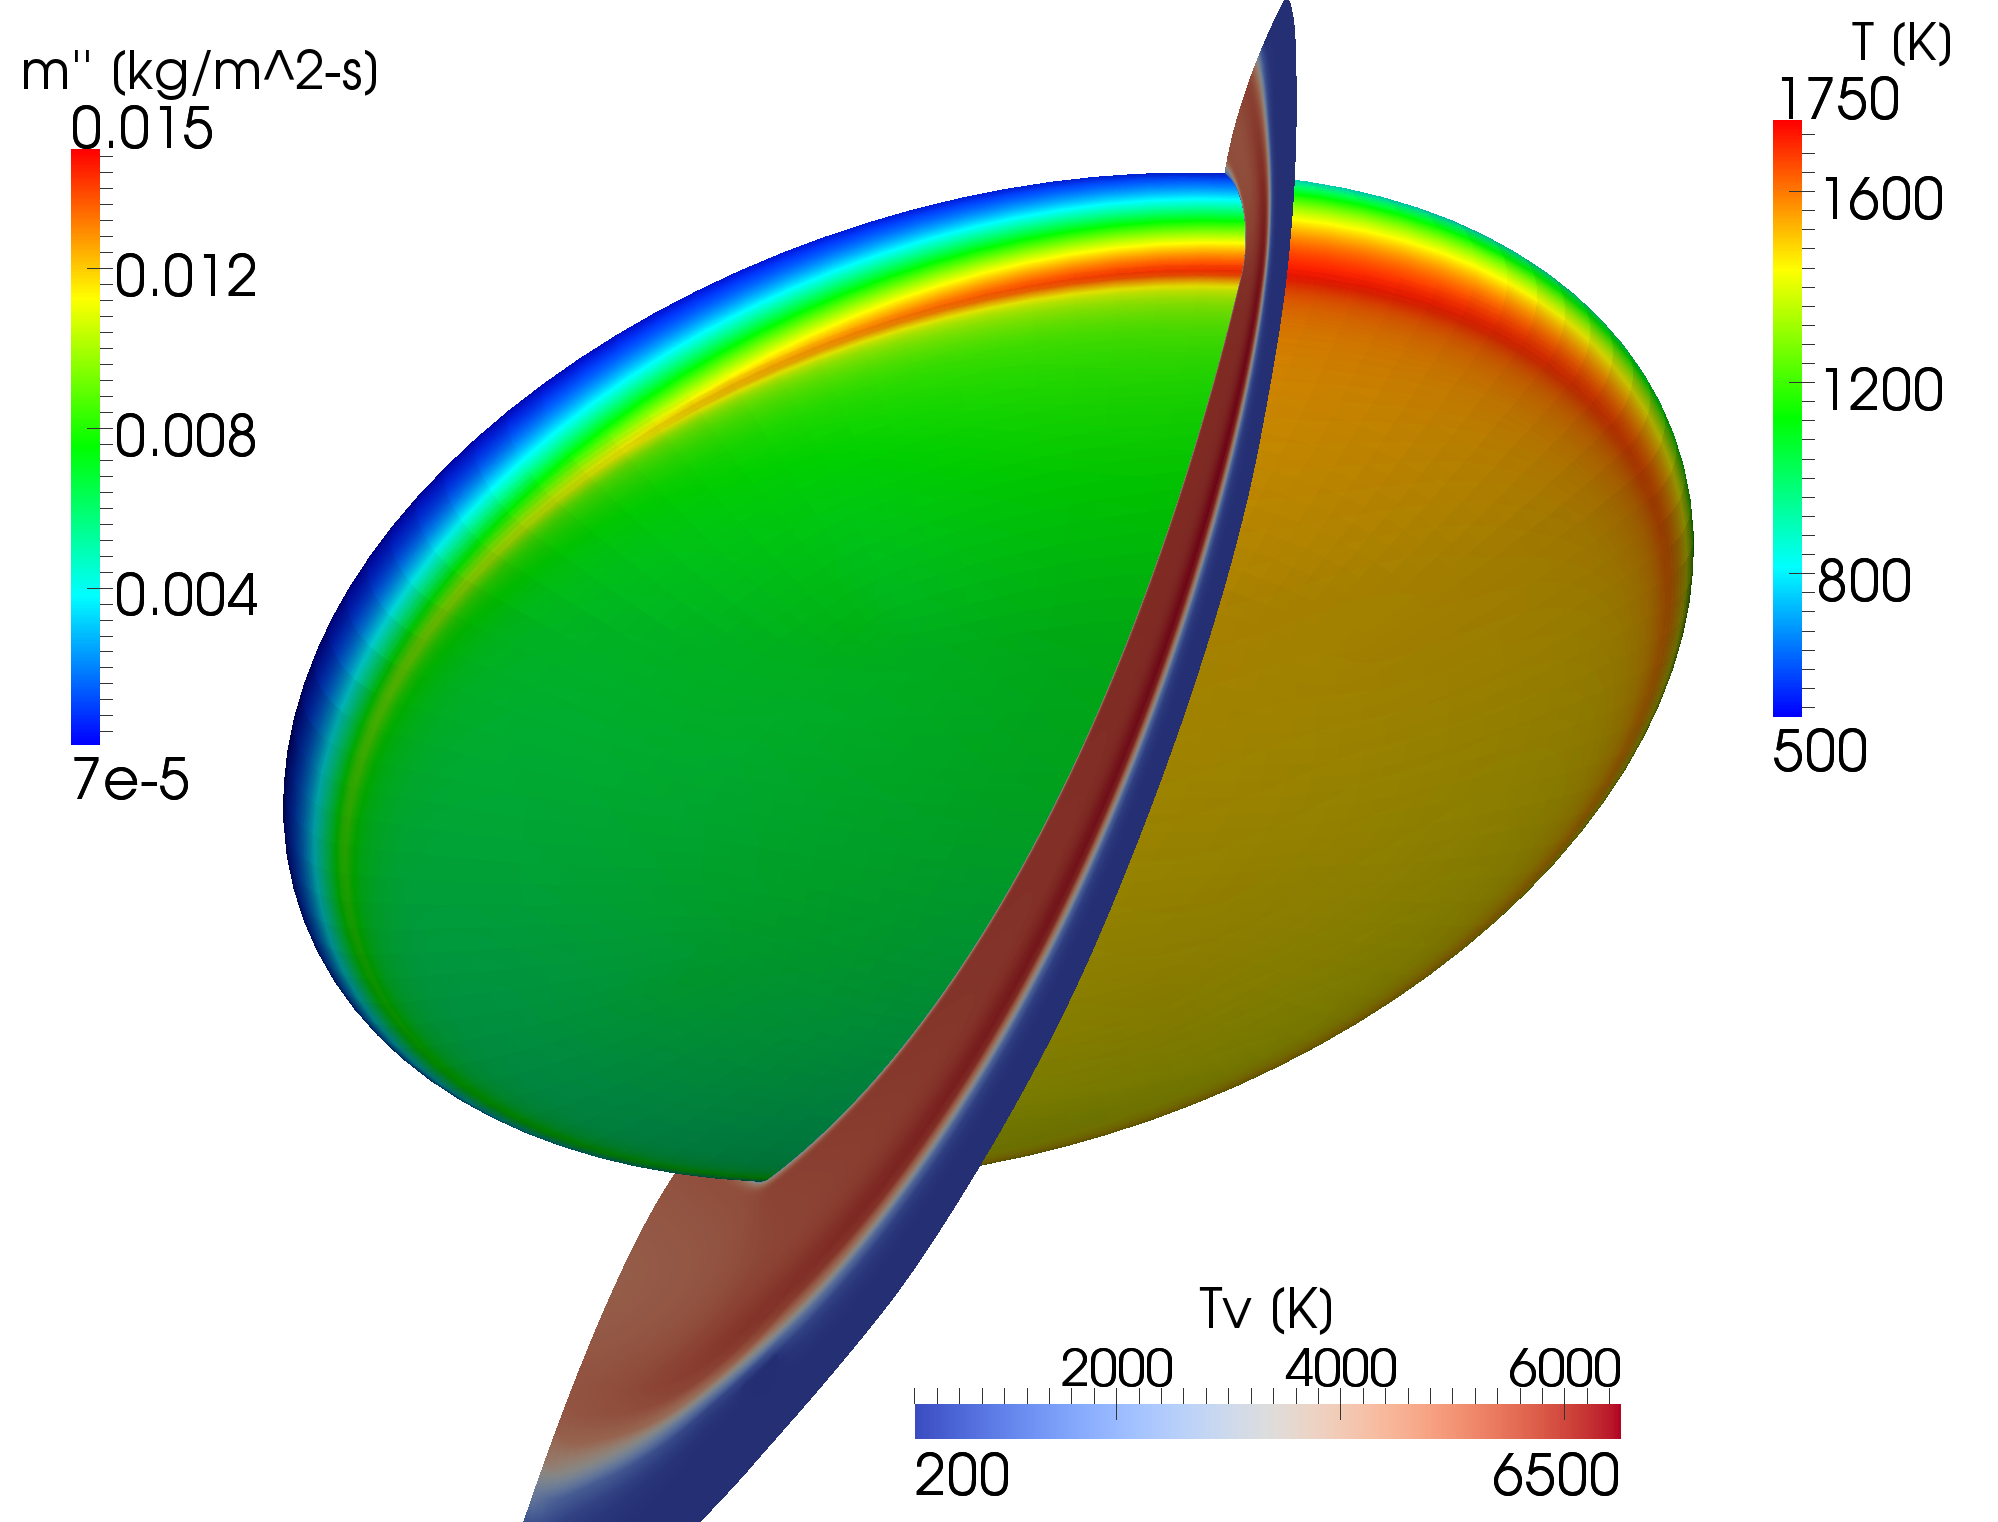
\includegraphics[width=.45\textwidth]{ablating_hs_wbg}
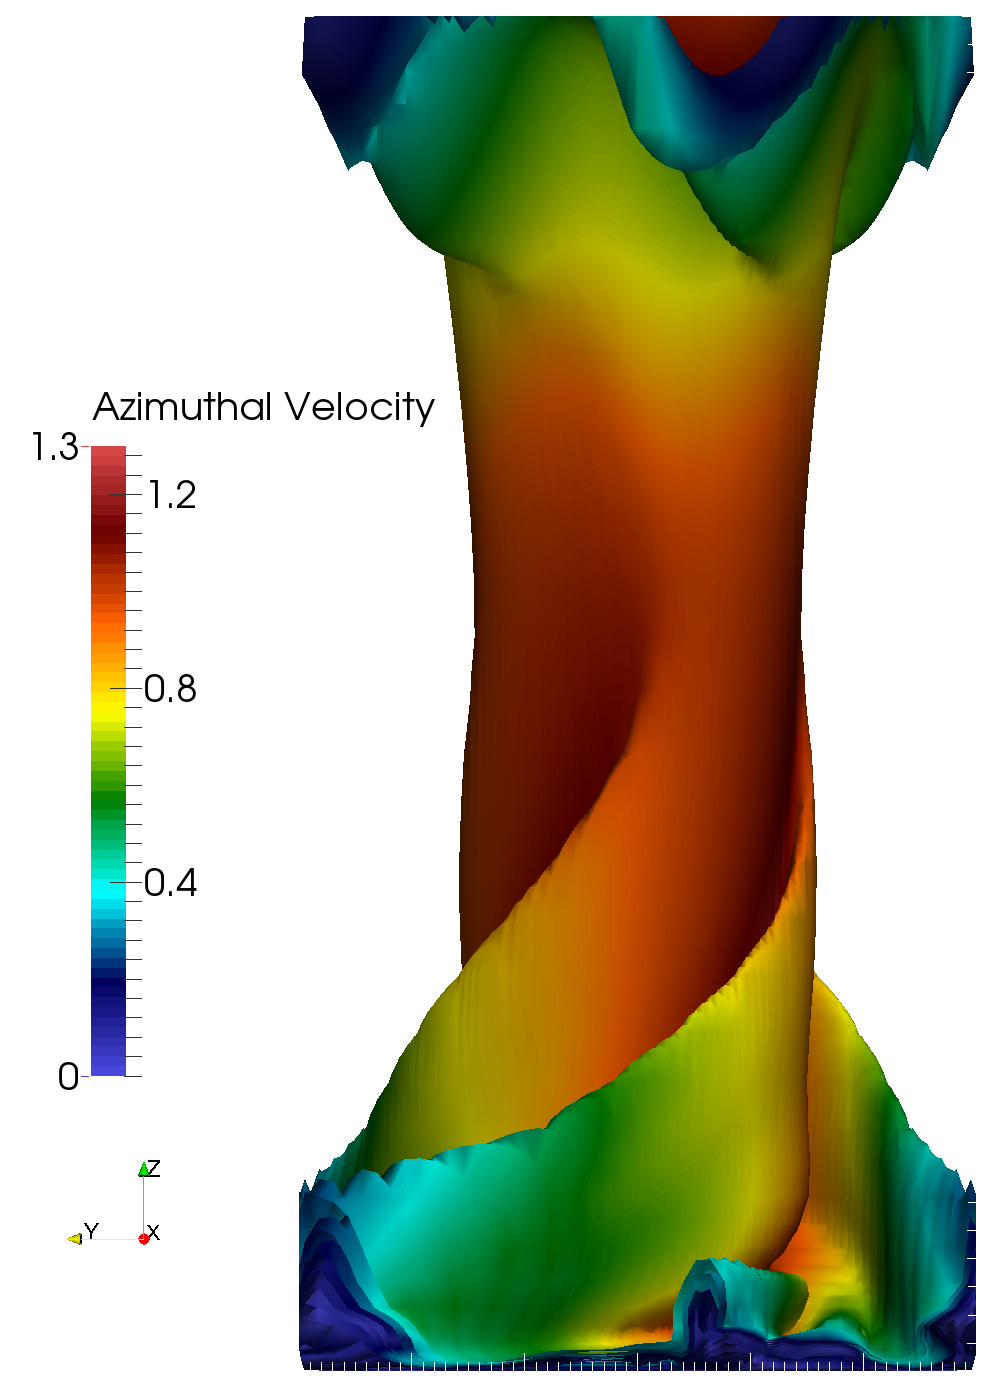
\includegraphics[width=.25\textwidth]{sov}
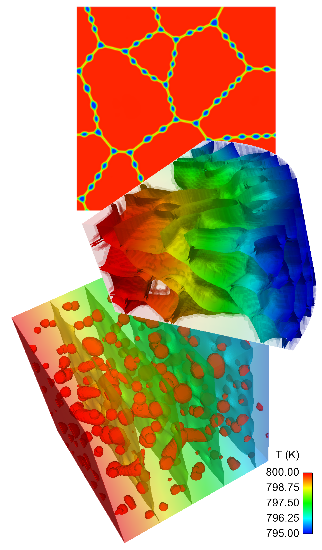
\includegraphics[width=.25\textwidth]{marmot1b}
\end{columns}

\begin{columns}
\column{.35\textwidth}
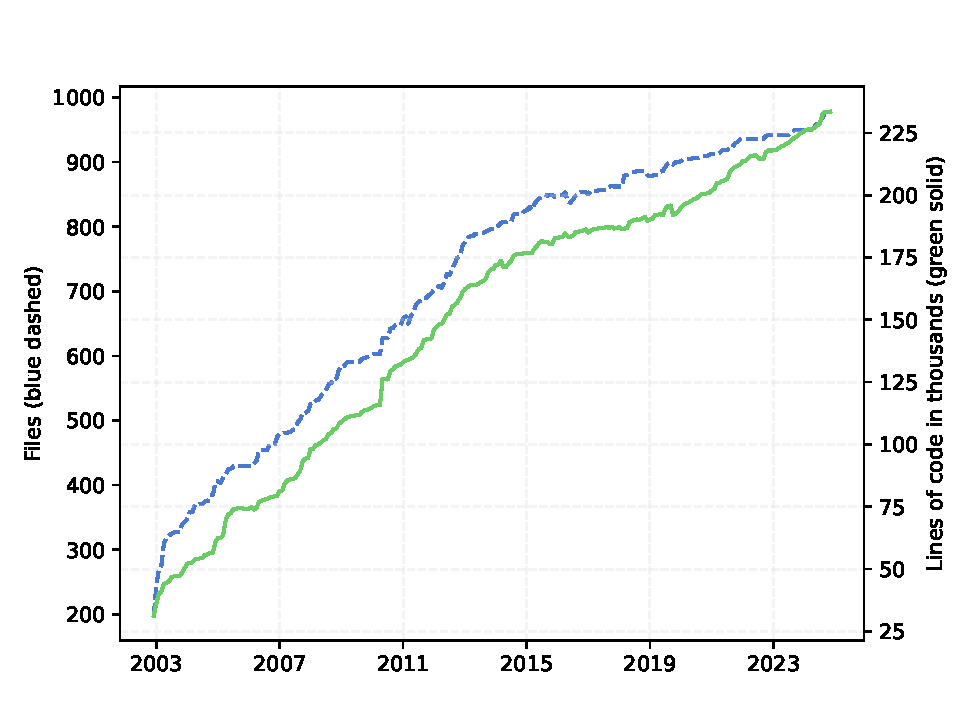
\includegraphics[width=\textwidth]{cloc_libmesh}

\column{.65\textwidth}
\begin{block}{Challenges}
\begin{itemize}
\item Radically different application types
\item Widely dispersed core developers
\begin{itemize}
\item At peak: INL, UT-Austin, U.Buffalo, JSC, MIT, Harvard, Argonne
\end{itemize}
\item OSS, commercial, private applications
\end{itemize}
\end{block}
\end{columns}

\end{frame}


\begin{frame}[t]
  \begin{columns}
    \column{.6\textwidth}
    \begin{center}
      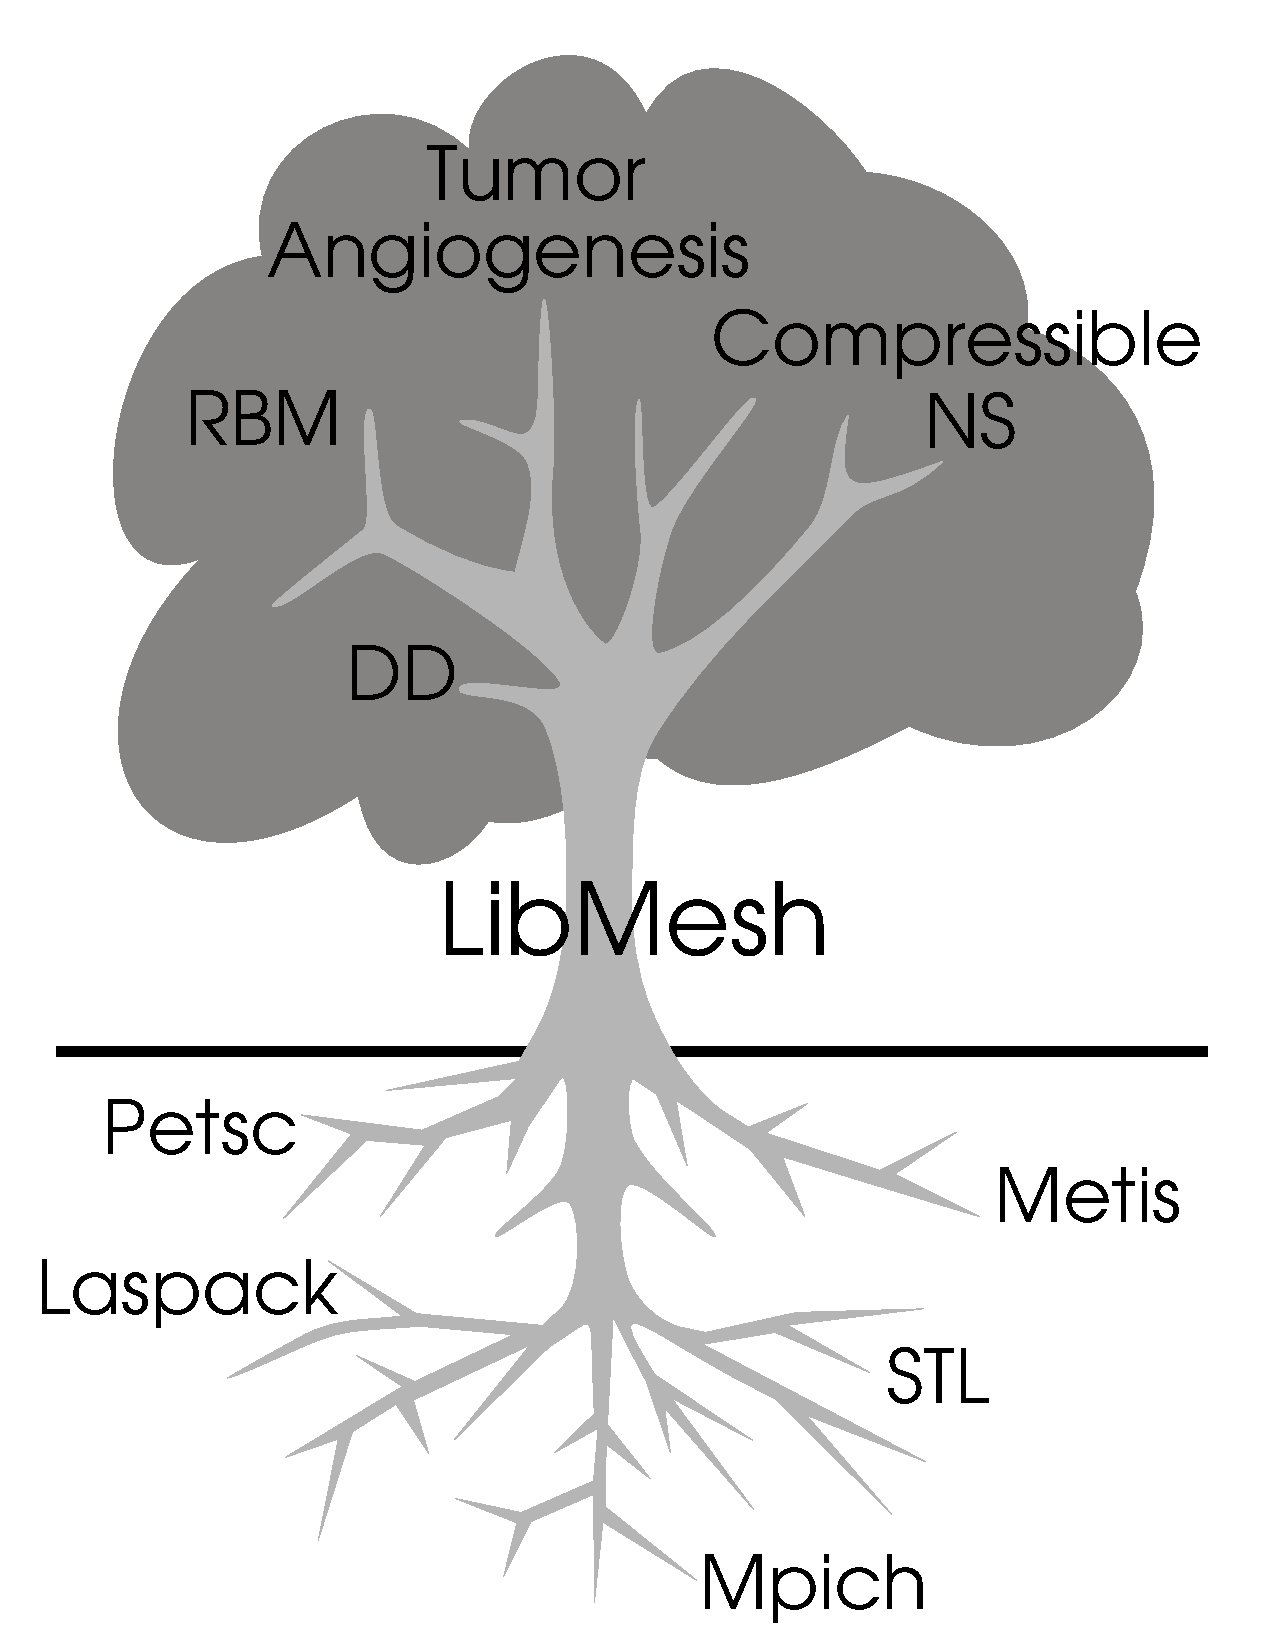
\includegraphics[width=.9\textwidth]{mytreeandroots_allnames}
    \end{center}
    \column{.35\textwidth}
    \begin{itemize}
      \item Foundational (typically optional) library access via LibMesh's ``roots''.
      \item Application ``branches'' built off the library ``trunk''.
      \item Additional middleware layers (e.g. Akselos, GRINS, MOOSE) for more complex applications
    \end{itemize}
  \end{columns}

\end{frame}



\section{Library Design}


\begin{frame}
\frametitle{Geometric Element Classes}

\begin{columns}
\column{.55\textwidth}
\begin{center}
\vspace{-5mm}
\includegraphics[width=.75\textwidth]{DofObjects}
\end{center}
\column{.45\textwidth}
\begin{itemize}
\item Abstract interface gives mesh topology
\item Concrete instantiations of mesh geometry
\item Hides element type from most applications
\item Runtime polymorphism allows mixed element types, dimensions
\item Base class data arrays allow more optimization, inlining
\end{itemize}

\end{columns}

\end{frame}


%%%%%%%%%%%%%%%%%%%%%%%%%%%%%%%%%%%%%%%%%%%%%%%%%
\frame
{
  \frametitle{Linear Algebra}
  \begin{center}
    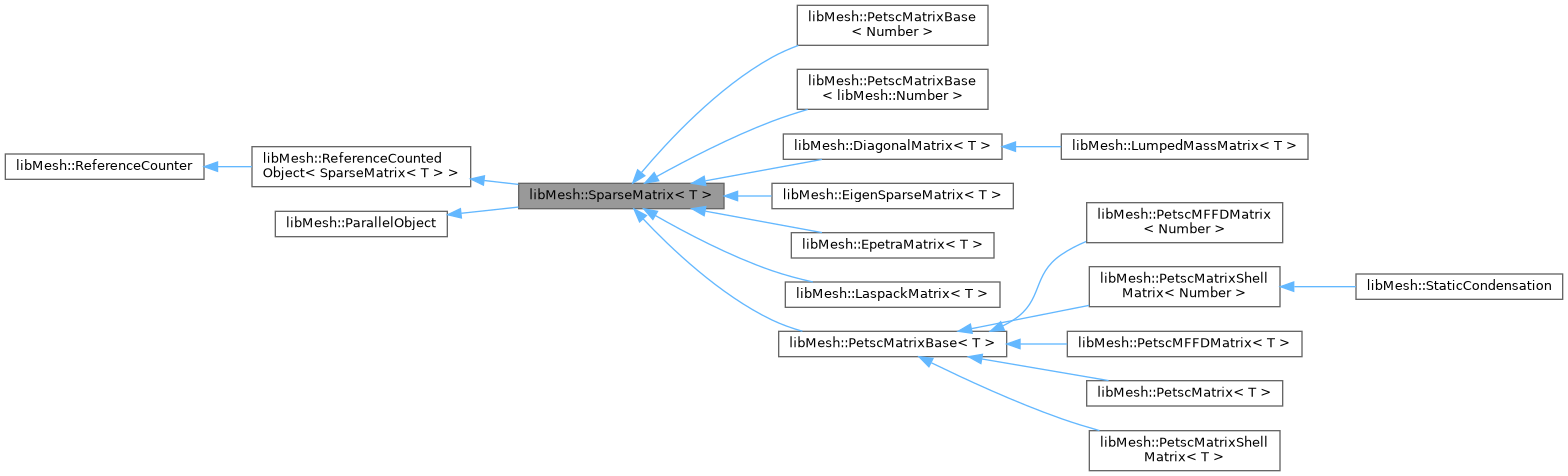
\includegraphics[width=\textwidth,trim=7.56in 0 0 0,clip]{classlibMesh_1_1SparseMatrix__inherit__graph}
  \end{center}
}



%%%%%%%%%%%%%%%%%%%%%%%%%%%%%%%%%%%%%%%%%%%%%%%%%
\frame
{
  \frametitle{I/O formats}
  \begin{center}
    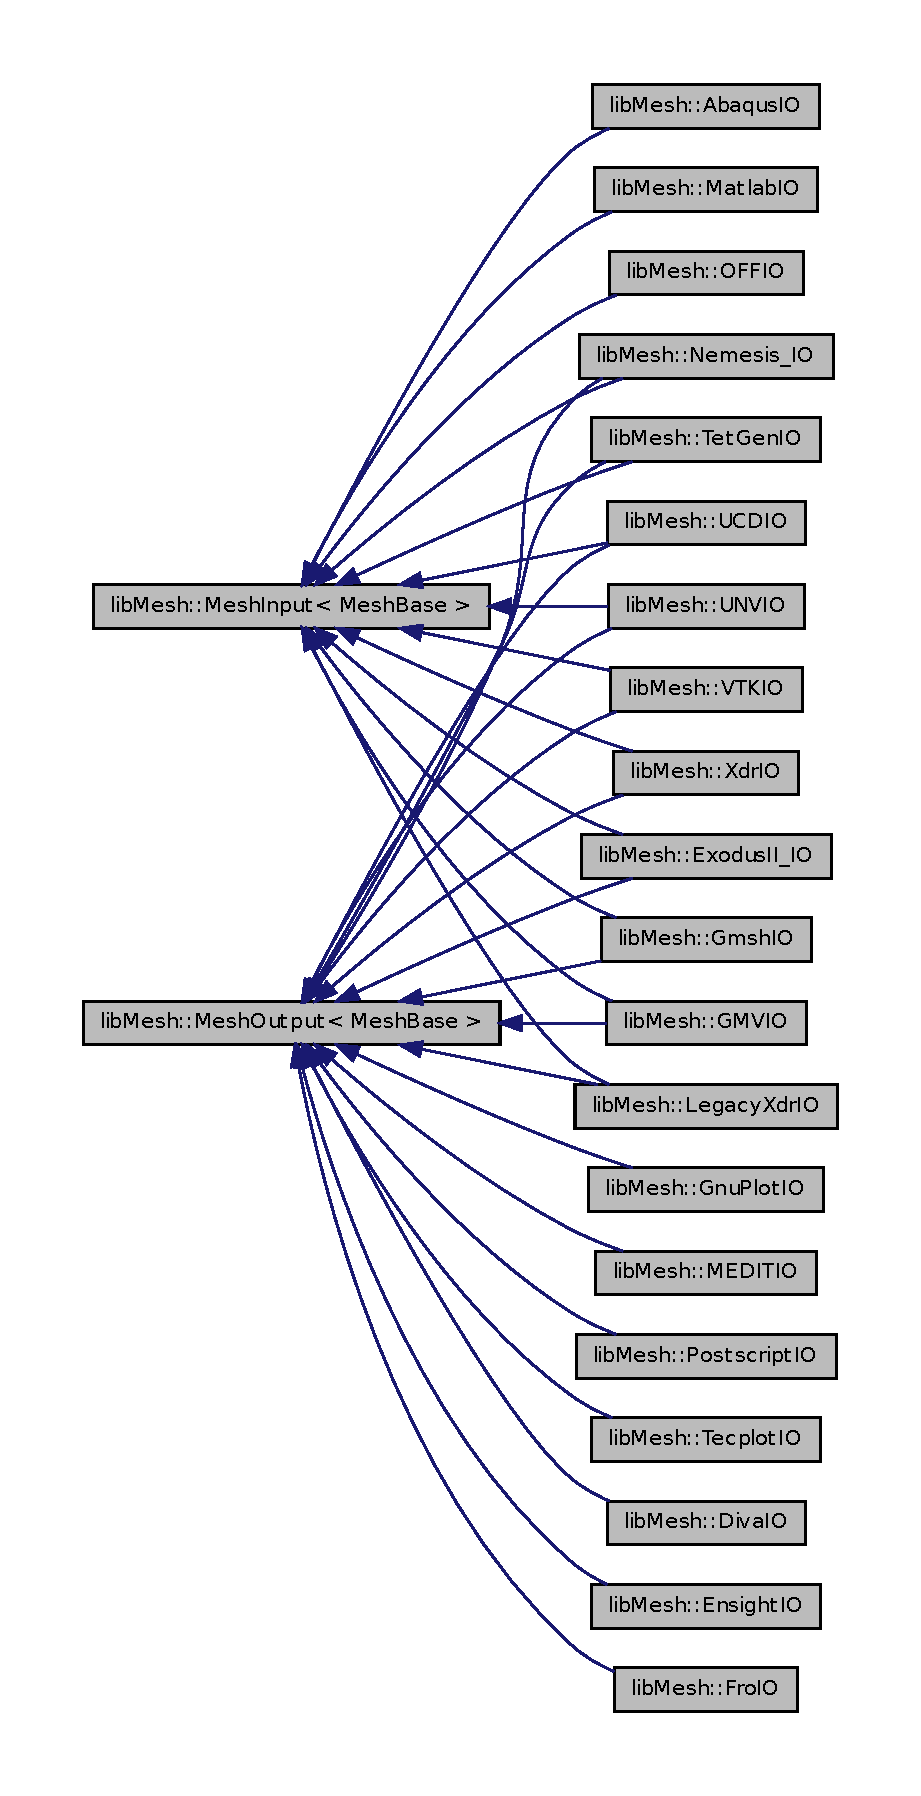
\includegraphics[height=0.9\textheight]{mesh_io}
  \end{center}
}


%%%%%%%%%%%%%%%%%%%%%%%%%%%%%%%%%%%%%%%%%%%%%%%%%
\frame
{
  \frametitle{Domain Partitioning}
  \begin{center}
    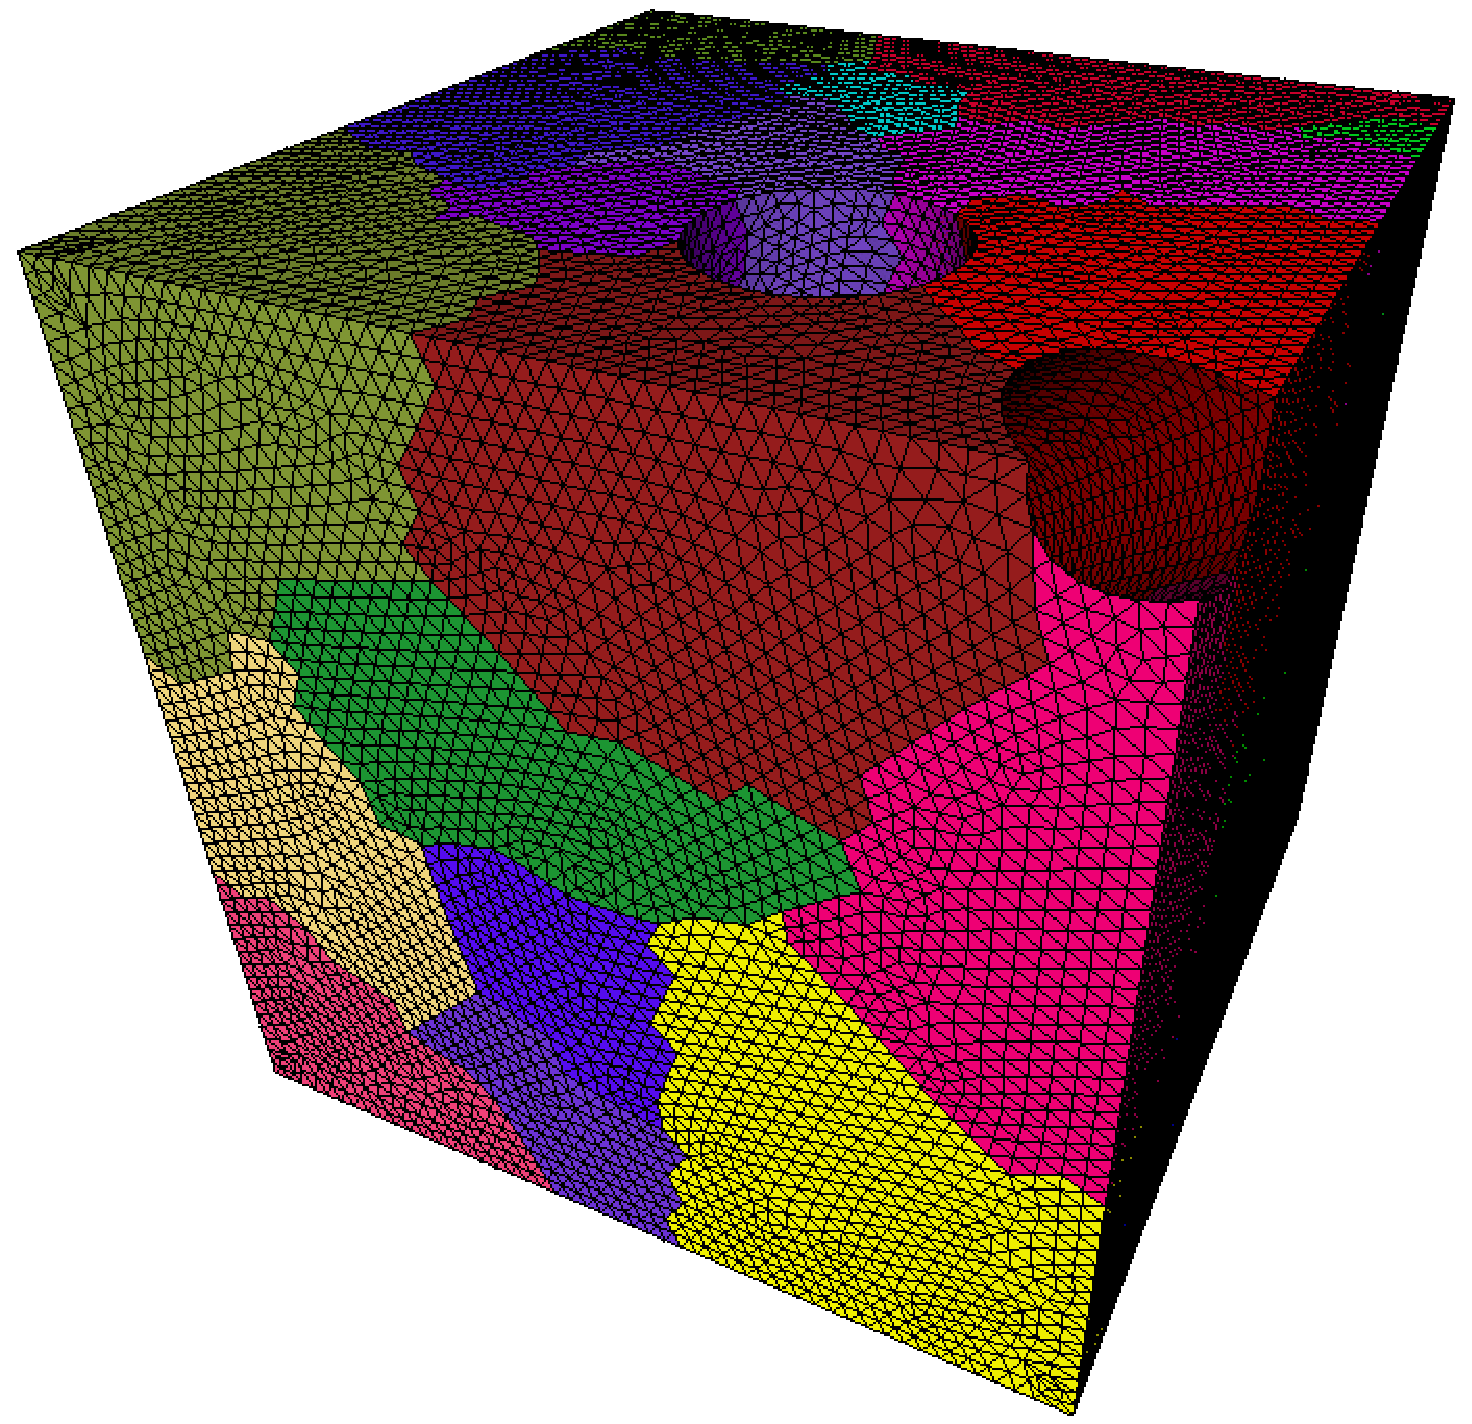
\includegraphics[width=.3\textwidth]{part_trans}
    %\\
    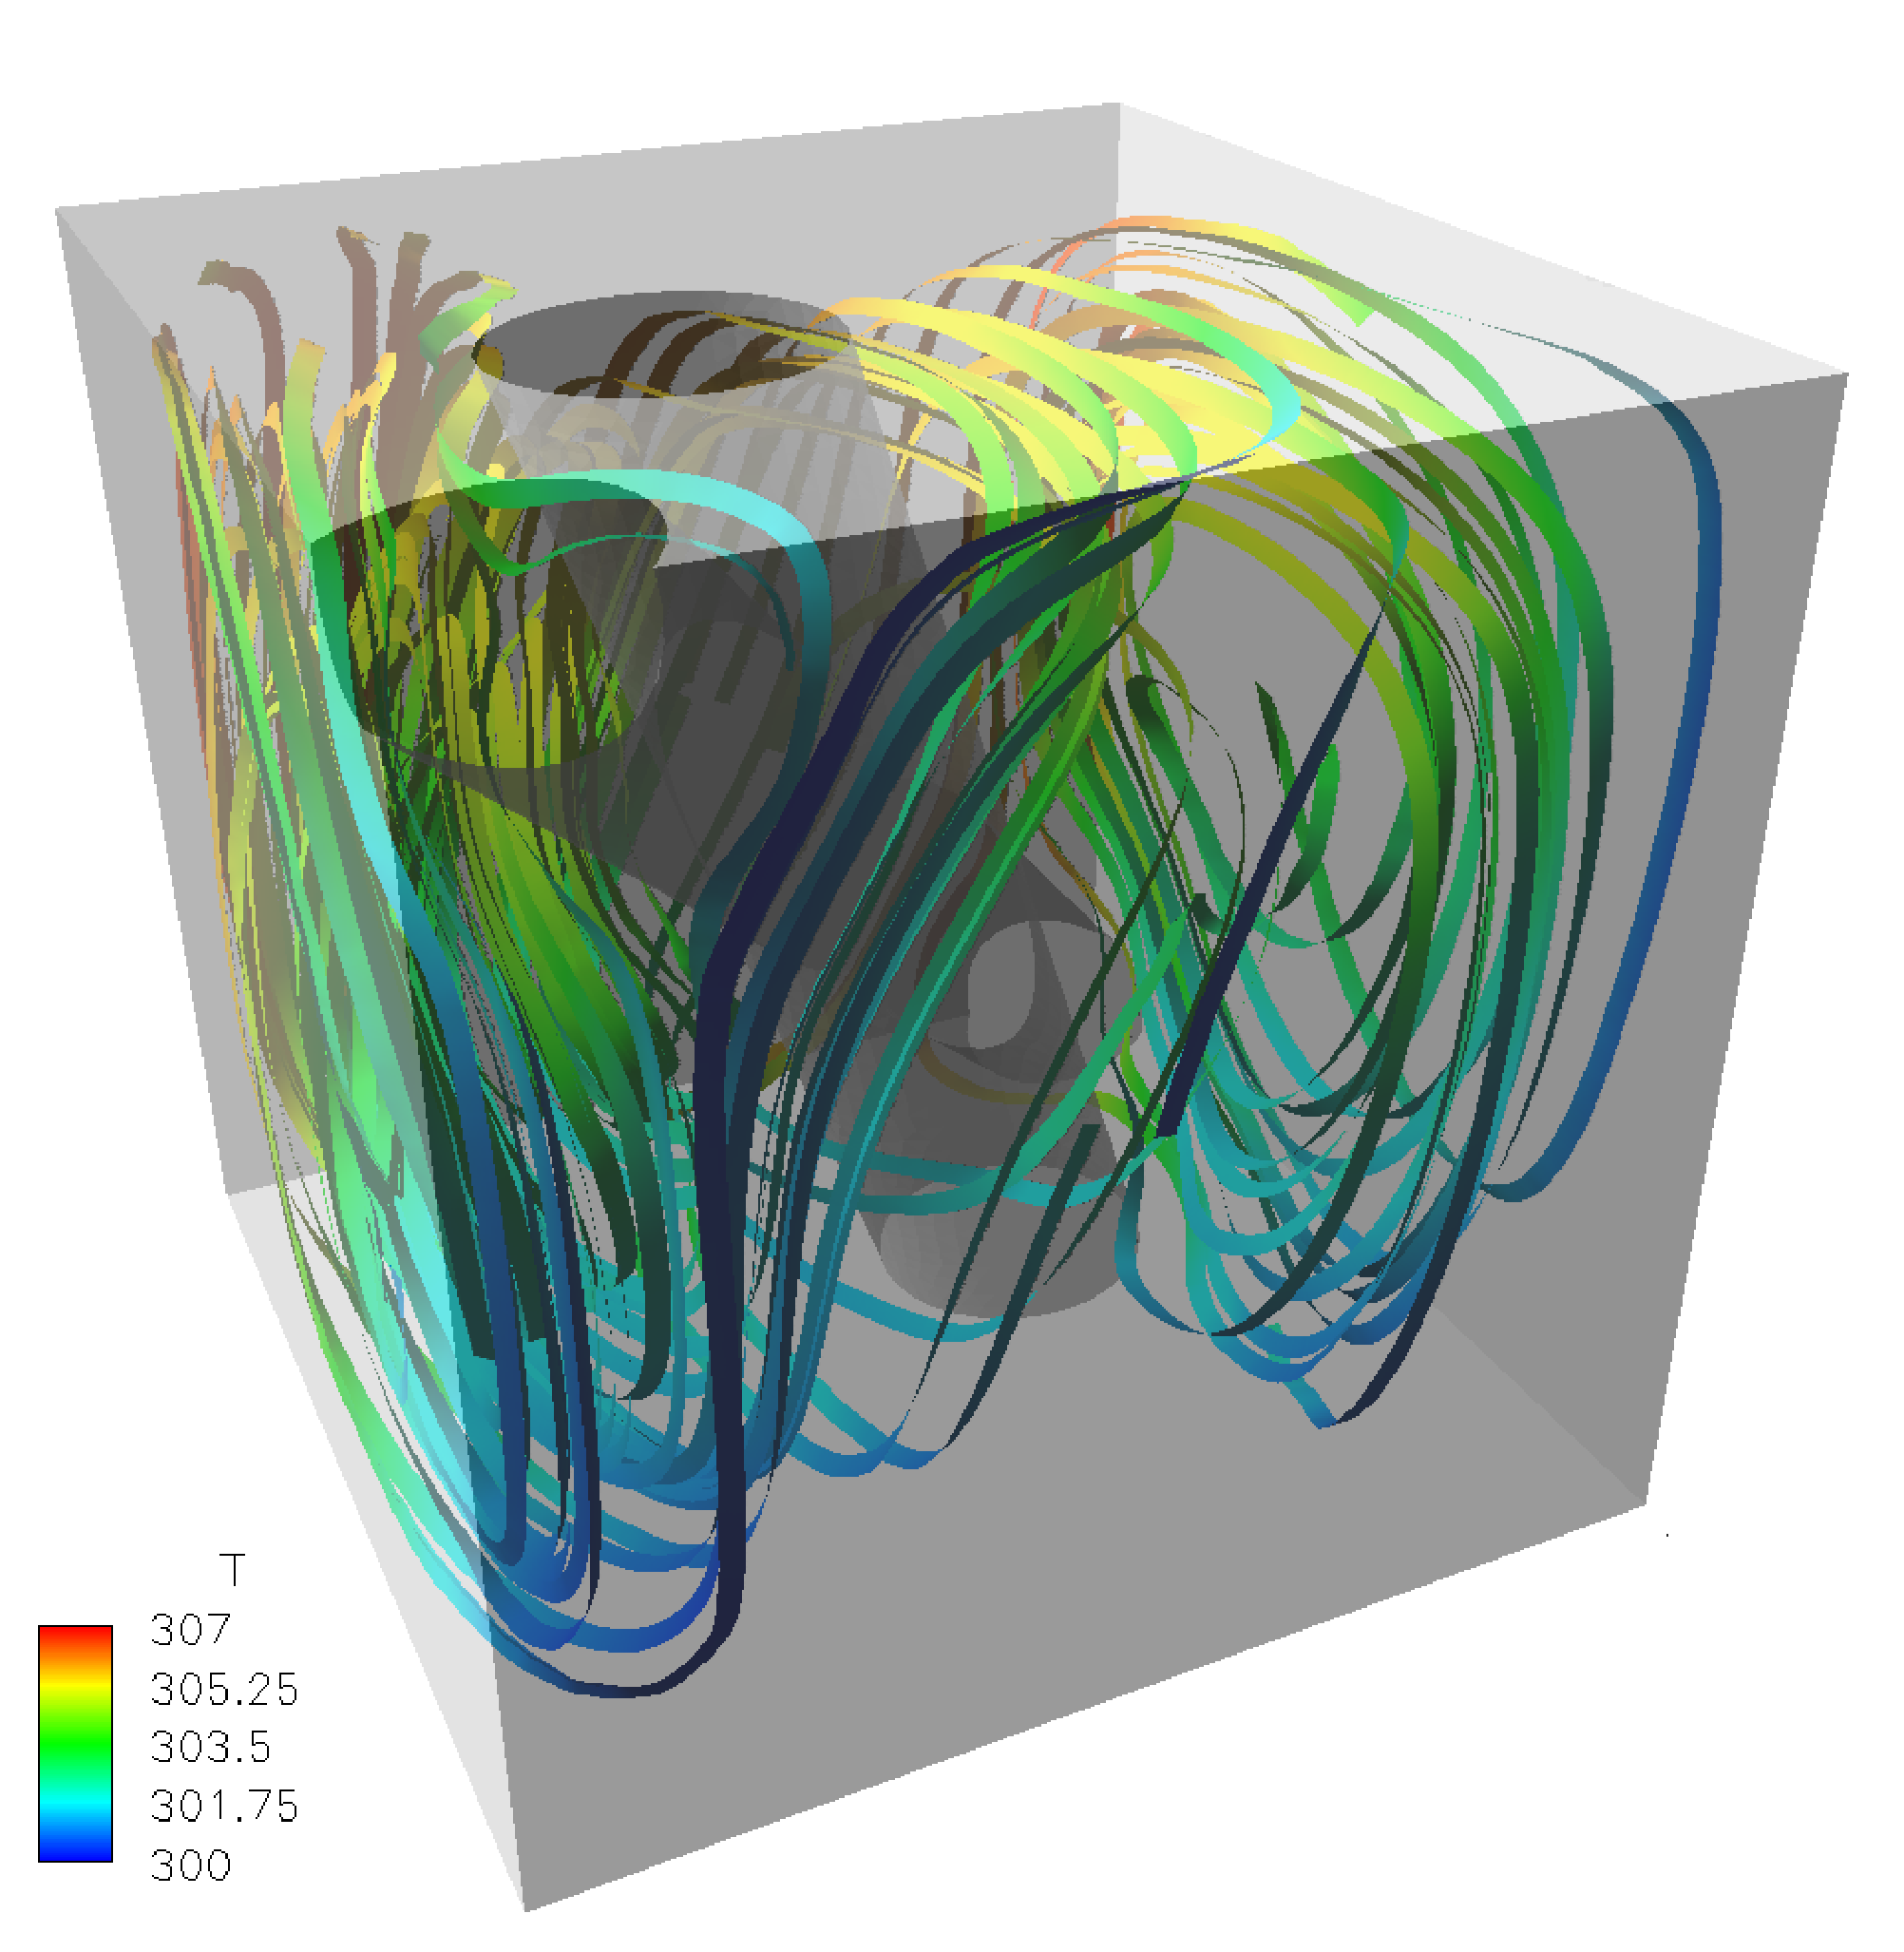
\includegraphics[width=.3\textwidth]{streamtraces}
  \end{center}  

  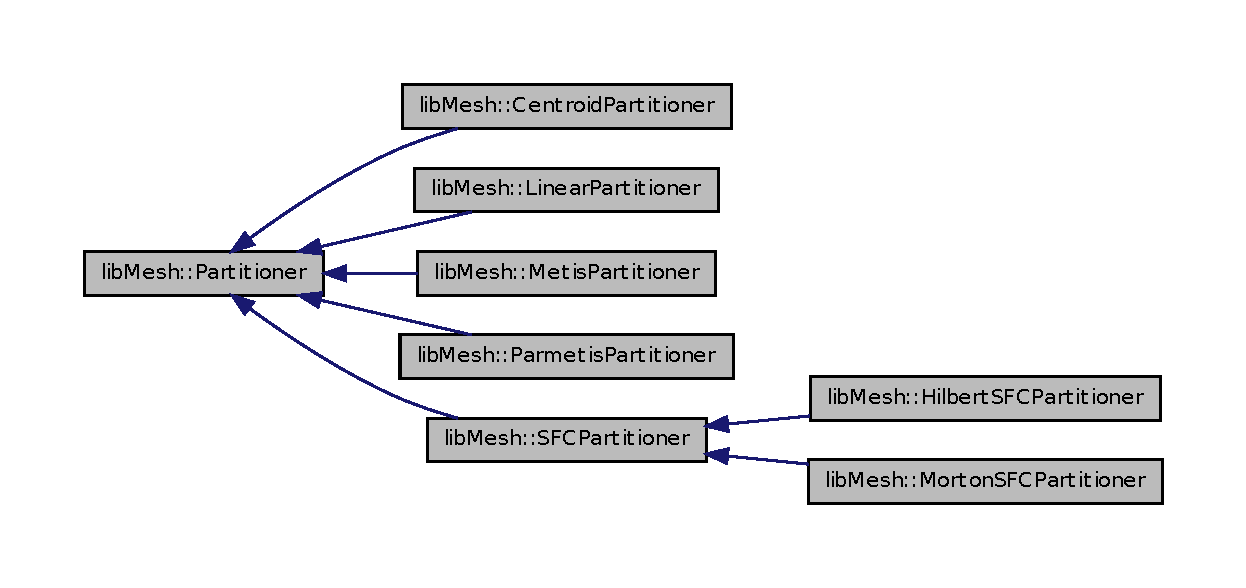
\includegraphics[width=.65\textwidth]{partitioner}
}


%%%%%%%%%%%%%%%%%%%%%%%%%%%%%%%%%%%%%%%%%%%%%%%%%
\begin{frame}
\frametitle{Mesh Data Structures}
\begin{columns}
\column{.6\textwidth}
\begin{center}
\includegraphics[width=.95\textwidth]{MeshUML}
\end{center}
\column{.4\textwidth}
%\begin{block}{}
\begin{itemize}
\item \texttt{MeshBase} gives node or element iterators, all vs active, global vs local
\item \texttt{ReplicatedMesh} or \texttt{DistributedMesh} manages synchronized or distributed data
\end{itemize}

\includegraphics[width=.75\textwidth]{ParallelMesh3}
%\end{block}
\end{columns}

\end{frame}



%%%%%%%%%%%%%%%%%%%%%%%%%%%%%%%%%%%%%%%%%%%%%%%%%
\frame
{
  \frametitle{Discretization: Finite Elements}
  \begin{center}
    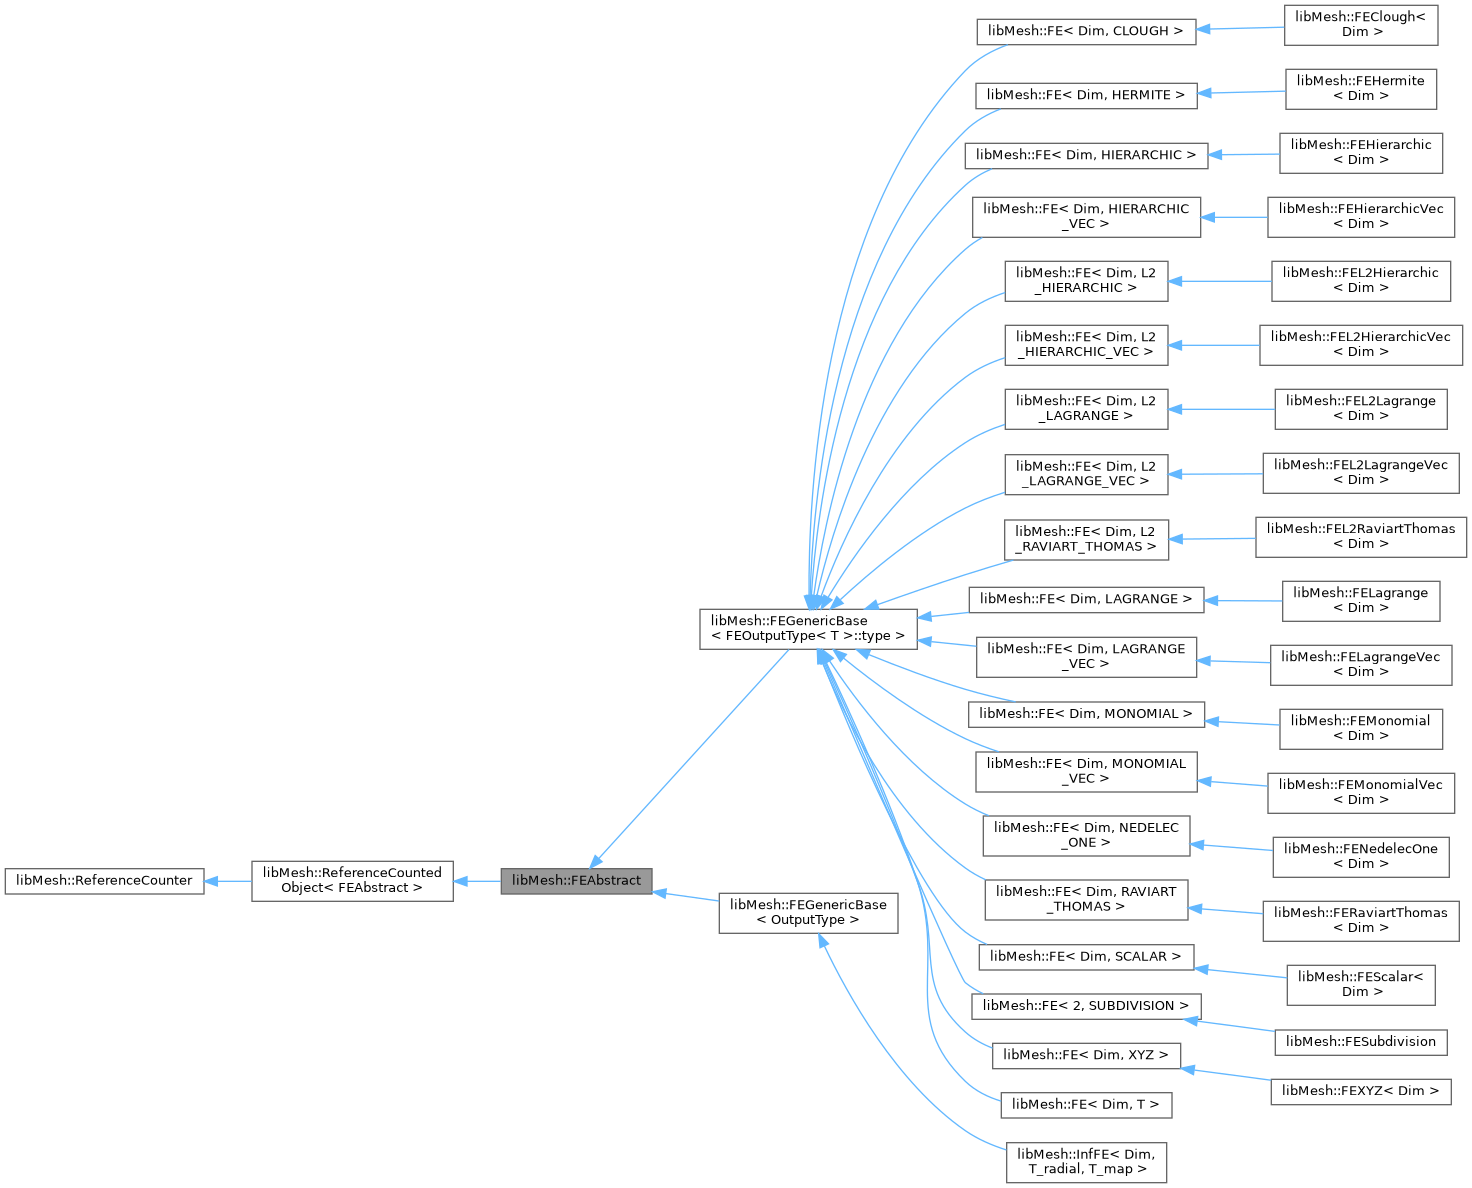
\includegraphics[width=0.9\textwidth,trim=7.4in 0 0 0,clip]{classlibMesh_1_1FEAbstract__inherit__graph}
  \end{center}
}      



%%%%%%%%%%%%%%%%%%%%%%%%%%%%%%%%%%%%%%%%%%%%%%%%%
\frame
{
  \frametitle{Algorithms: Error Estimation}
  \begin{center}
    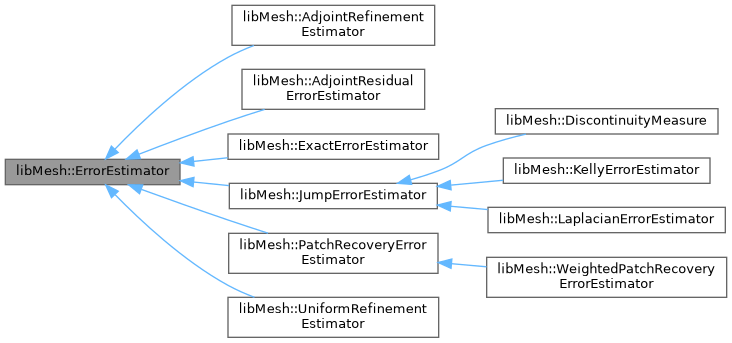
\includegraphics[width=\textwidth]{classlibMesh_1_1ErrorEstimator__inherit__graph}
  \end{center}
}



% \input{physics_codes}
% \input{software_development}
\section{Boundary Value Problems}
%%%%%%%%%%%%%%%%%%%%%%%%%%%%%%%%%%%%%%%%%%%%%%%%%

\subsection*{A Generic BVP}

\begin{frame}[t]
  \begin{columns}[t]
    \column{.5\textwidth}
     \begin{itemize}
      \item Common BVP components:
      \vspace{-.1in}
        \begin{eqnarray}
        \label{eqn:general_pde}
        \nonumber
        \bv{M} \frac{\partial \bv{u}}{\partial t} & = & \bv{F}( \bv{u} ) \;\, \in \Omega \subset \Reals^n
        \\
        \nonumber
        \bv{G}( \bv{u} ) & = & 0 \;\;\;\;\;\;\;\; \in \Omega
        \\
        \nonumber
        \bv{u} & = & \bv{u}_D \;\;\;\;\; \in \partial \Omega_D
        \\
        \nonumber
        \bv{N}(\bv{u}) & = & 0 \;\;\;\;\;\;\;\; \in \partial \Omega_N
        \\
        \nonumber
        \bv{u}(\bv{x}, 0) & = & u_0(\bv{x}) 
      \end{eqnarray}
      \item Less common components:
        \begin{itemize}
        \item Moving domain $\Omega(t)$, $\Omega(\bv{u},t)$
        \item Multi-dimensional manifolds
        \item Self-overlapping, contact
        \item Acceleration ${\partial^2 u}/{\partial t^2}$
        \item Integro-differential equations
        \end{itemize}
      \end{itemize}
    \column{.5\textwidth}
      \begin{center}
        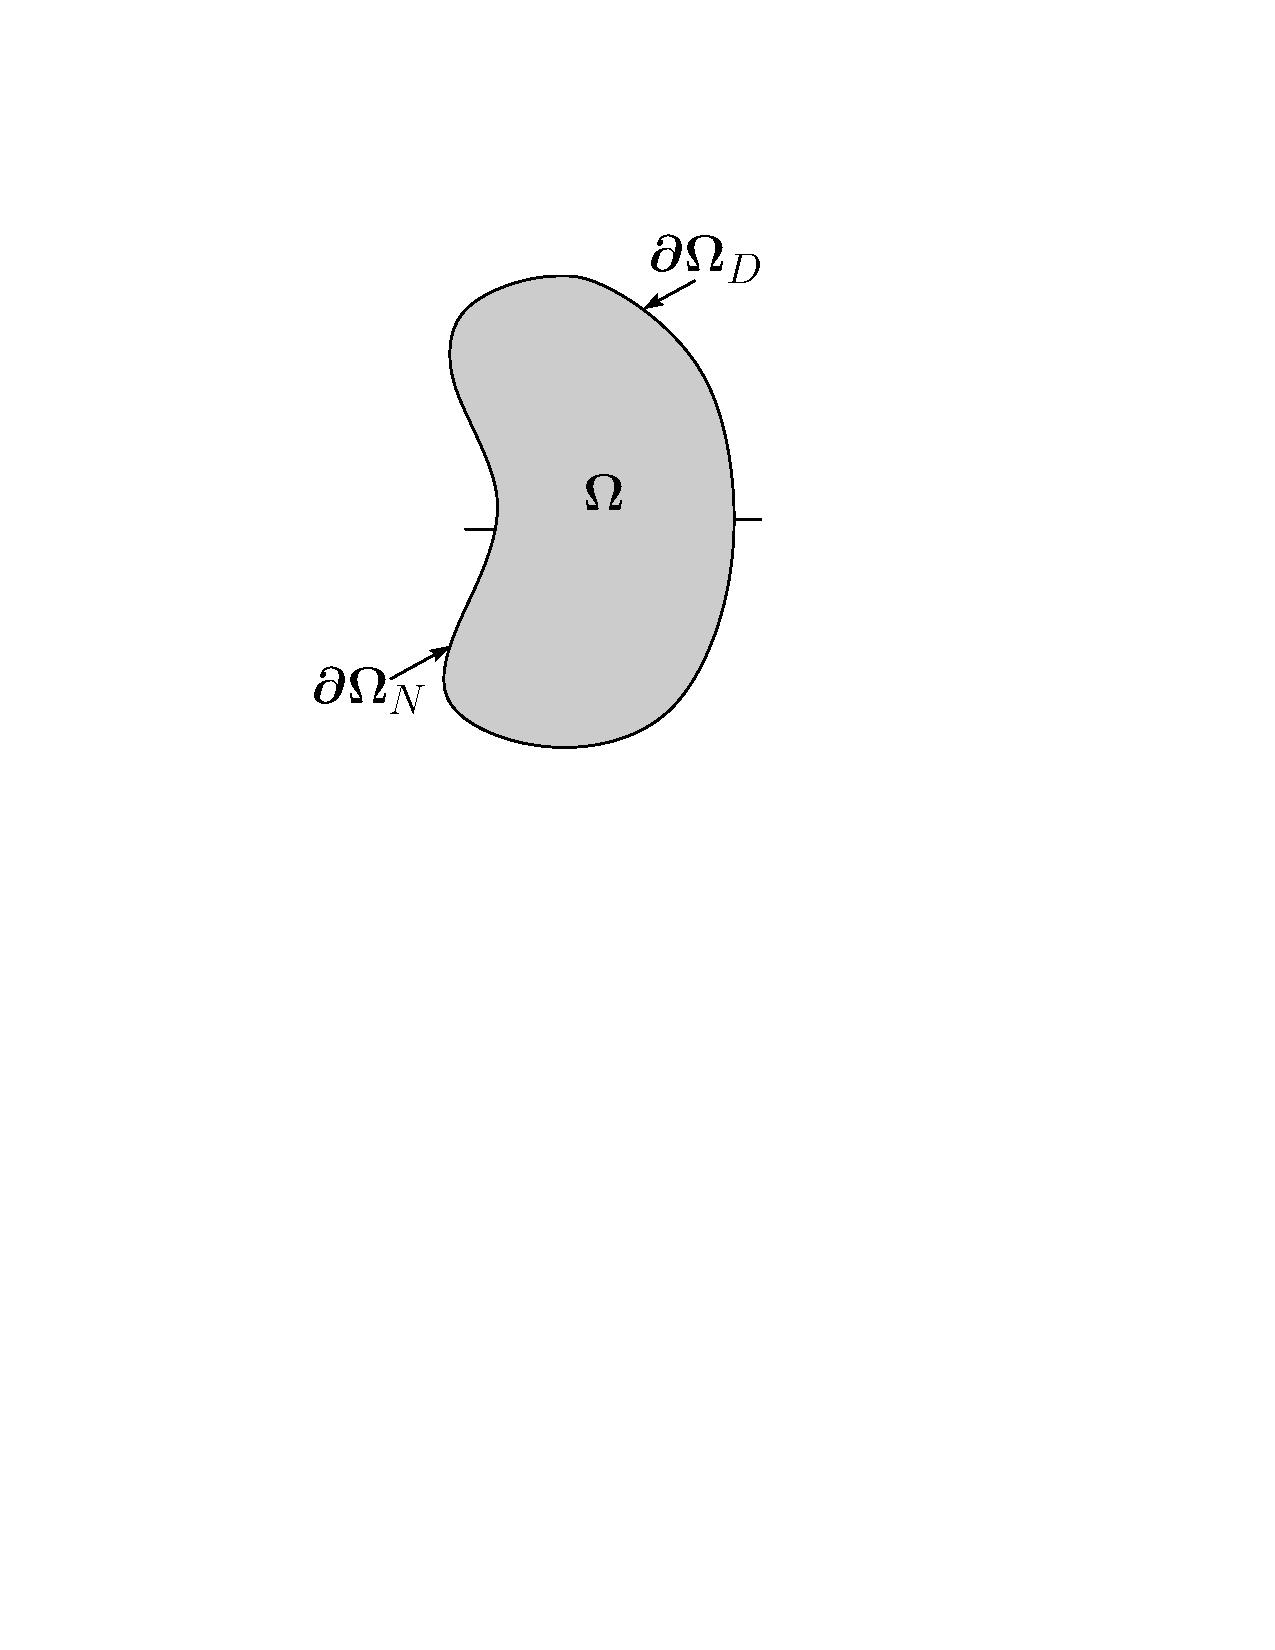
\includegraphics[viewport=140 420 400 685,clip=true,width=.45\textwidth]{domain2_input}
        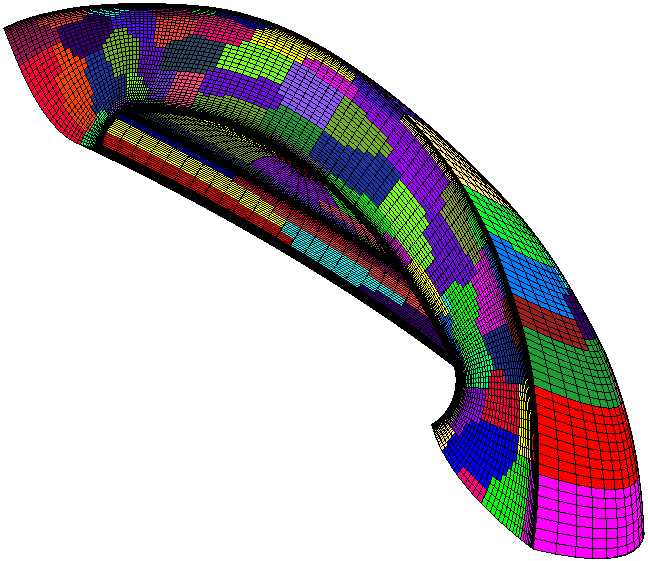
\includegraphics[width=.45\textwidth]{capsule_partitioned}

        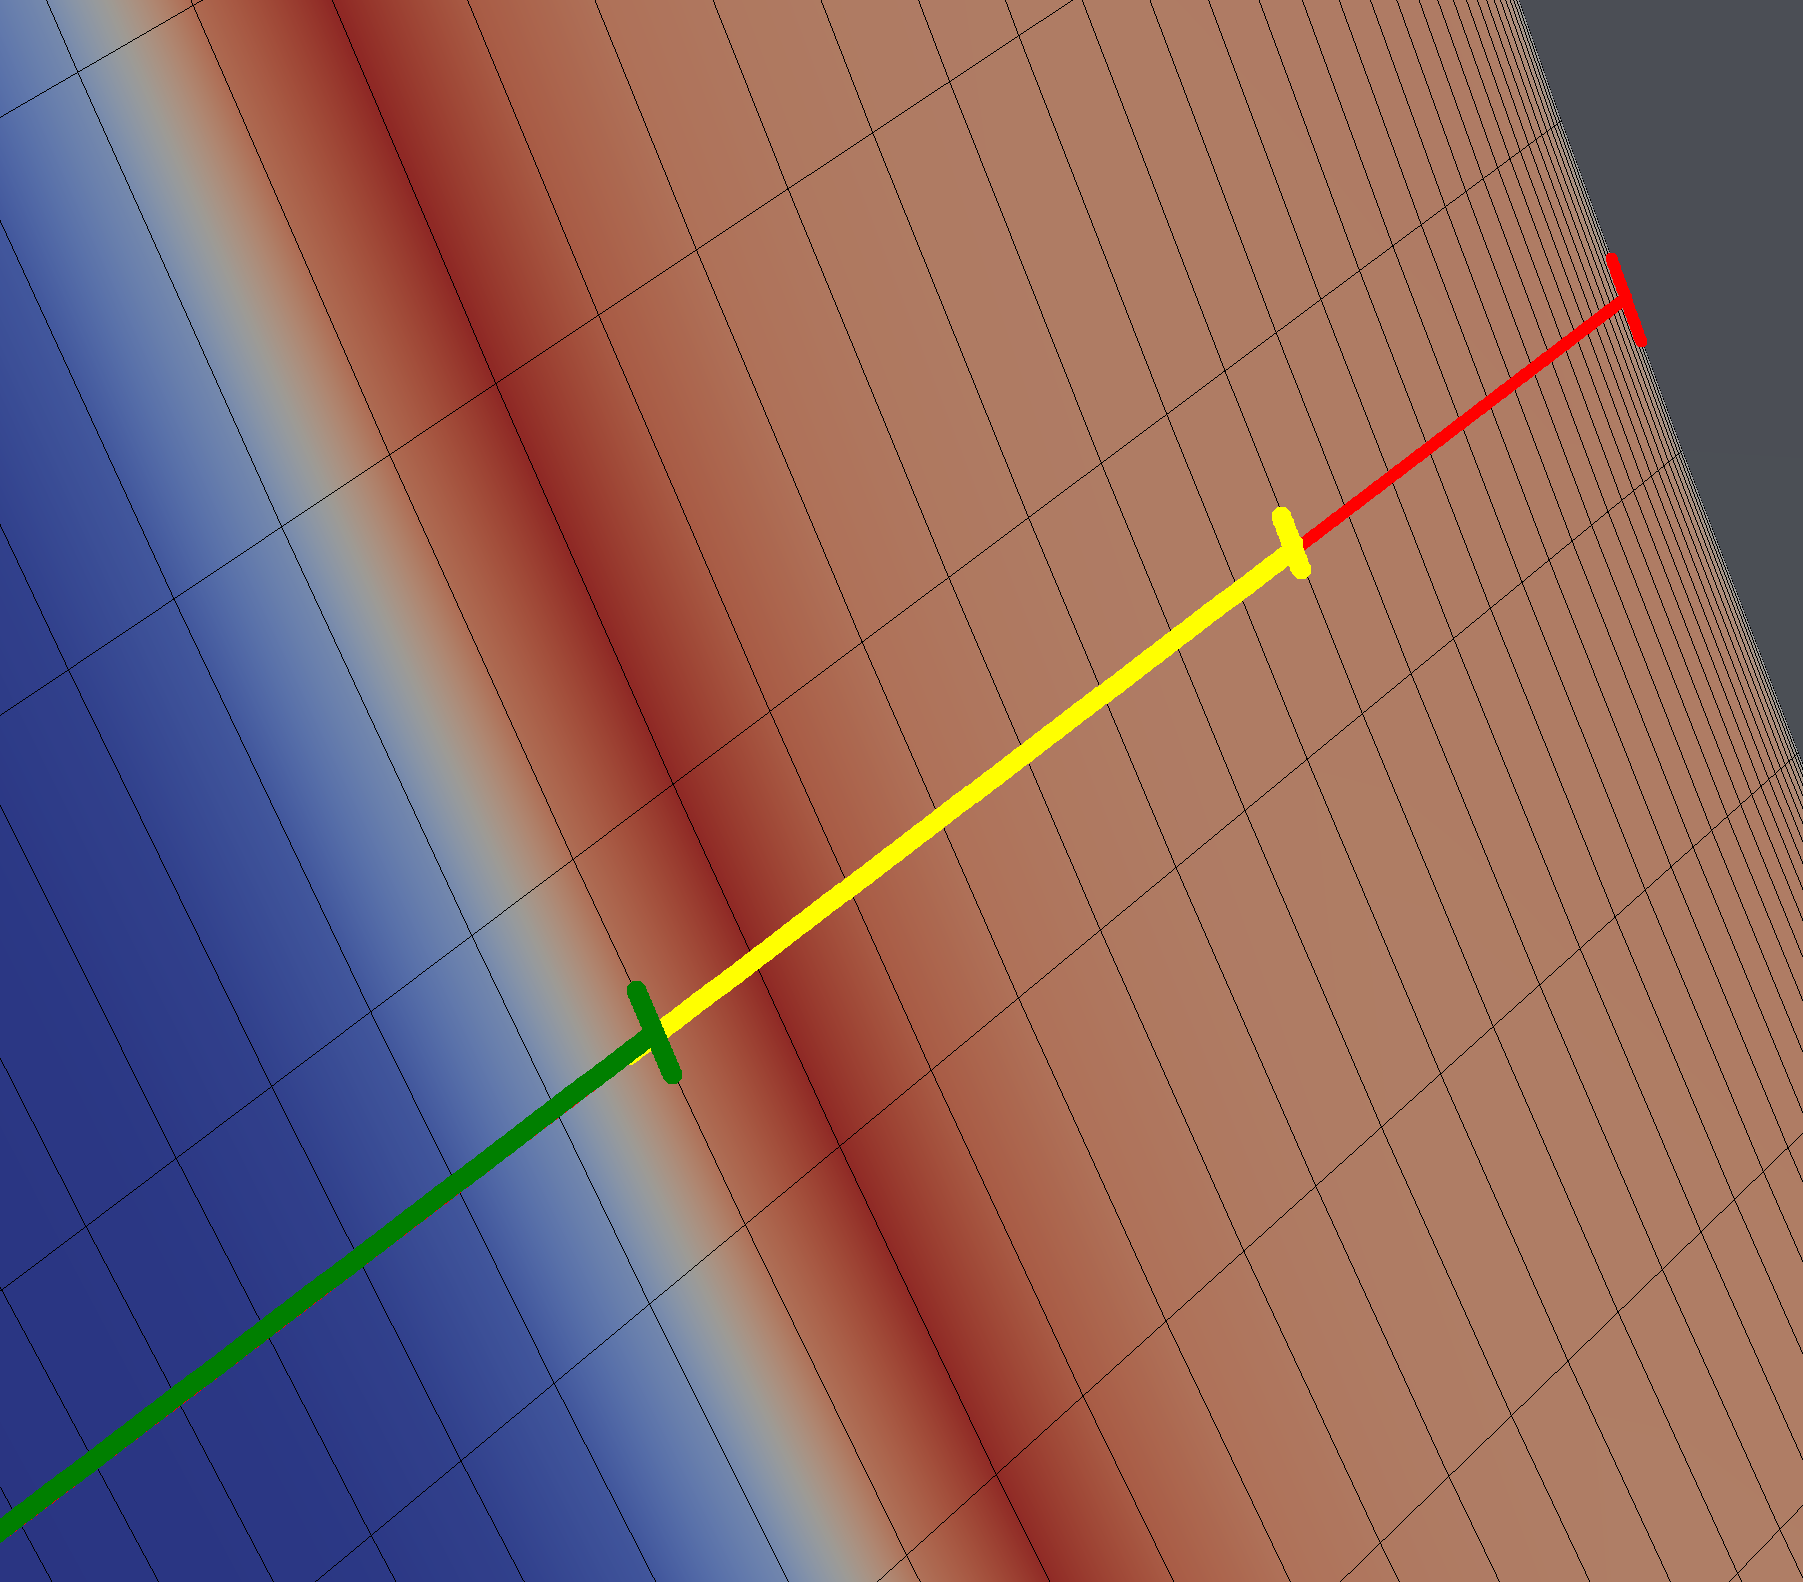
\includegraphics[width=.45\textwidth]{fins-transition} \;
        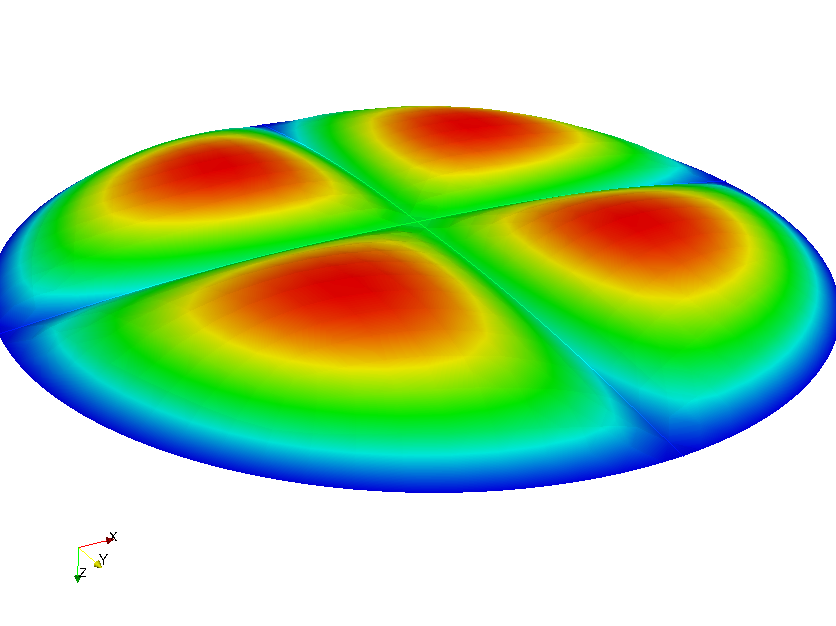
\includegraphics[width=.45\textwidth]{sheet_perspective}

      \end{center}
  \end{columns}
\end{frame}


\begin{frame}
  %\frametitle{}
  \begin{columns}[t]
    \column{.5\textwidth}
    \begin{block}{}%A general class of PDE}
      \begin{itemize}
      \item{
	Associated to the problem domain $\Omega$ is a \libMesh{} data
	structure accessed through a \texttt{MeshBase}
      }

      \item{A \texttt{Mesh} is essentially
	a collection of finite elements}
      \end{itemize}
      \begin{equation}
	\label{eqn:discretized_domain}
	\nonumber
	\Omega^h:=\bigcup_e \Omega_e
      \end{equation}
    \end{block}
    %\pause
    \column{.5\textwidth}
    %\begin{block}{}
      \begin{center}
	%\fbox{
	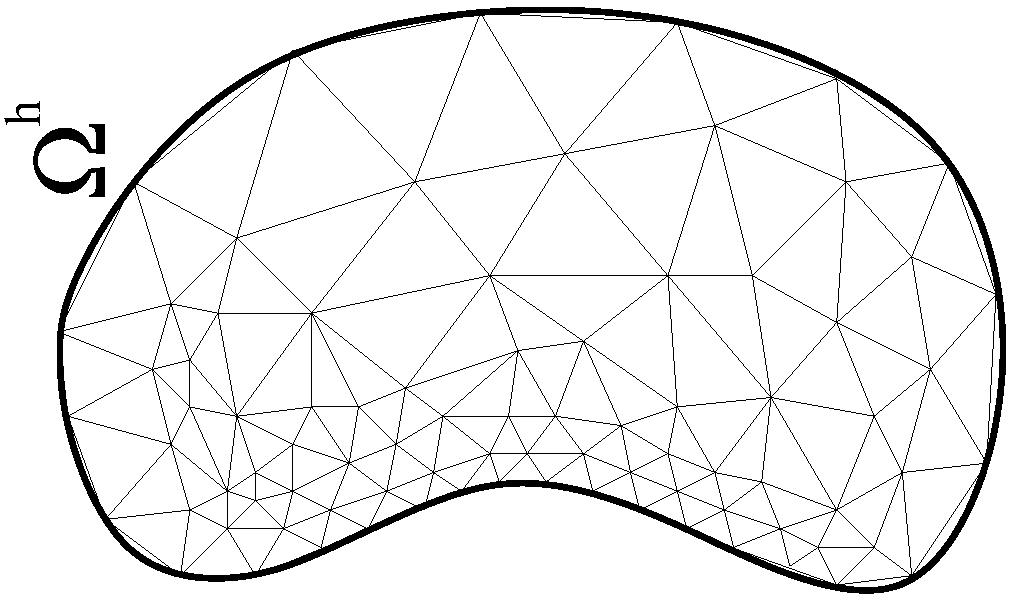
\includegraphics[width=2in,angle=-90]{discretized_domain}
	%}
      \end{center}
    %\end{block}
  \end{columns}
  \visible<2>
  {
  \begin{itemize}
    \item{\libMesh{} provides some simple structured mesh generation
routines, interfaces to Triangle, TetGen, Poly2Tri and Netgen, and read support for many input file formats.}
  \end{itemize}
  }
\end{frame}


\section{Object-Oriented Library Design}


\begin{frame}
\frametitle{Geometric Element Classes}

\begin{columns}
\column{.55\textwidth}
\begin{center}
\vspace{-5mm}
\includegraphics[width=.75\textwidth]{DofObjects}
\end{center}
\column{.45\textwidth}
\begin{itemize}
\item Abstract interface gives mesh topology
\item Concrete instantiations of mesh geometry
\item Hides element type from most applications
\item Runtime polymorphism allows mixed element types, dimensions
\item Base class data arrays allow more optimization, inlining
\end{itemize}

\end{columns}

\end{frame}


%%%%%%%%%%%%%%%%%%%%%%%%%%%%%%%%%%%%%%%%%%%%%%%%%
\frame
{
  \frametitle{Linear Algebra}
  \begin{center}
    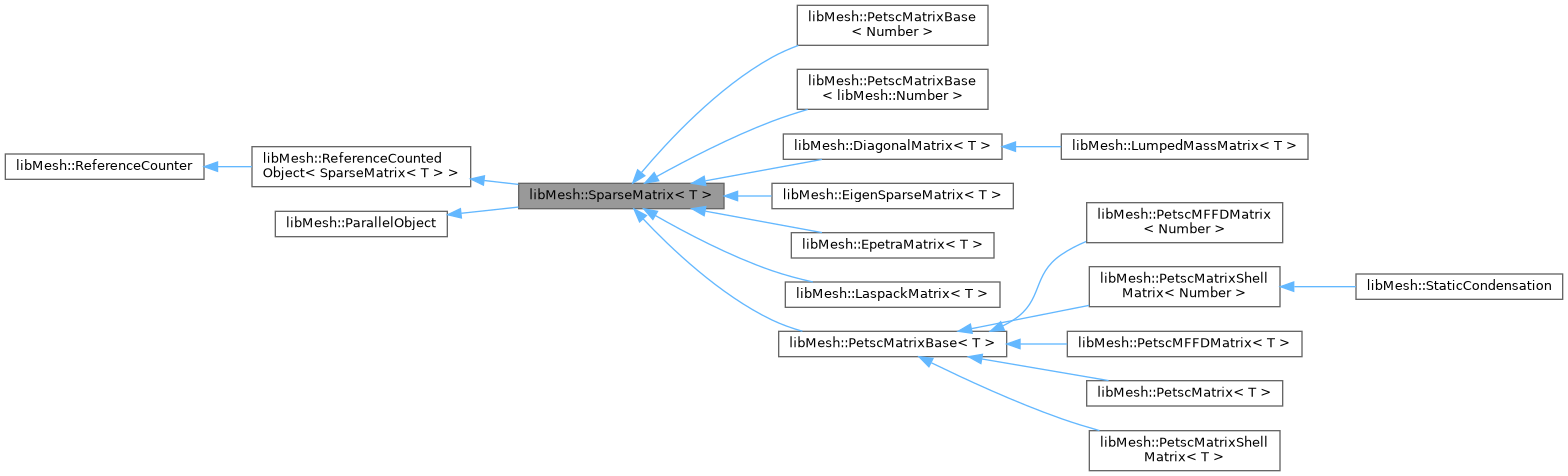
\includegraphics[width=\textwidth,trim=7.56in 0 0 0,clip]{classlibMesh_1_1SparseMatrix__inherit__graph}
  \end{center}
}



%%%%%%%%%%%%%%%%%%%%%%%%%%%%%%%%%%%%%%%%%%%%%%%%%
\frame
{
  \frametitle{I/O formats}
  \begin{center}
    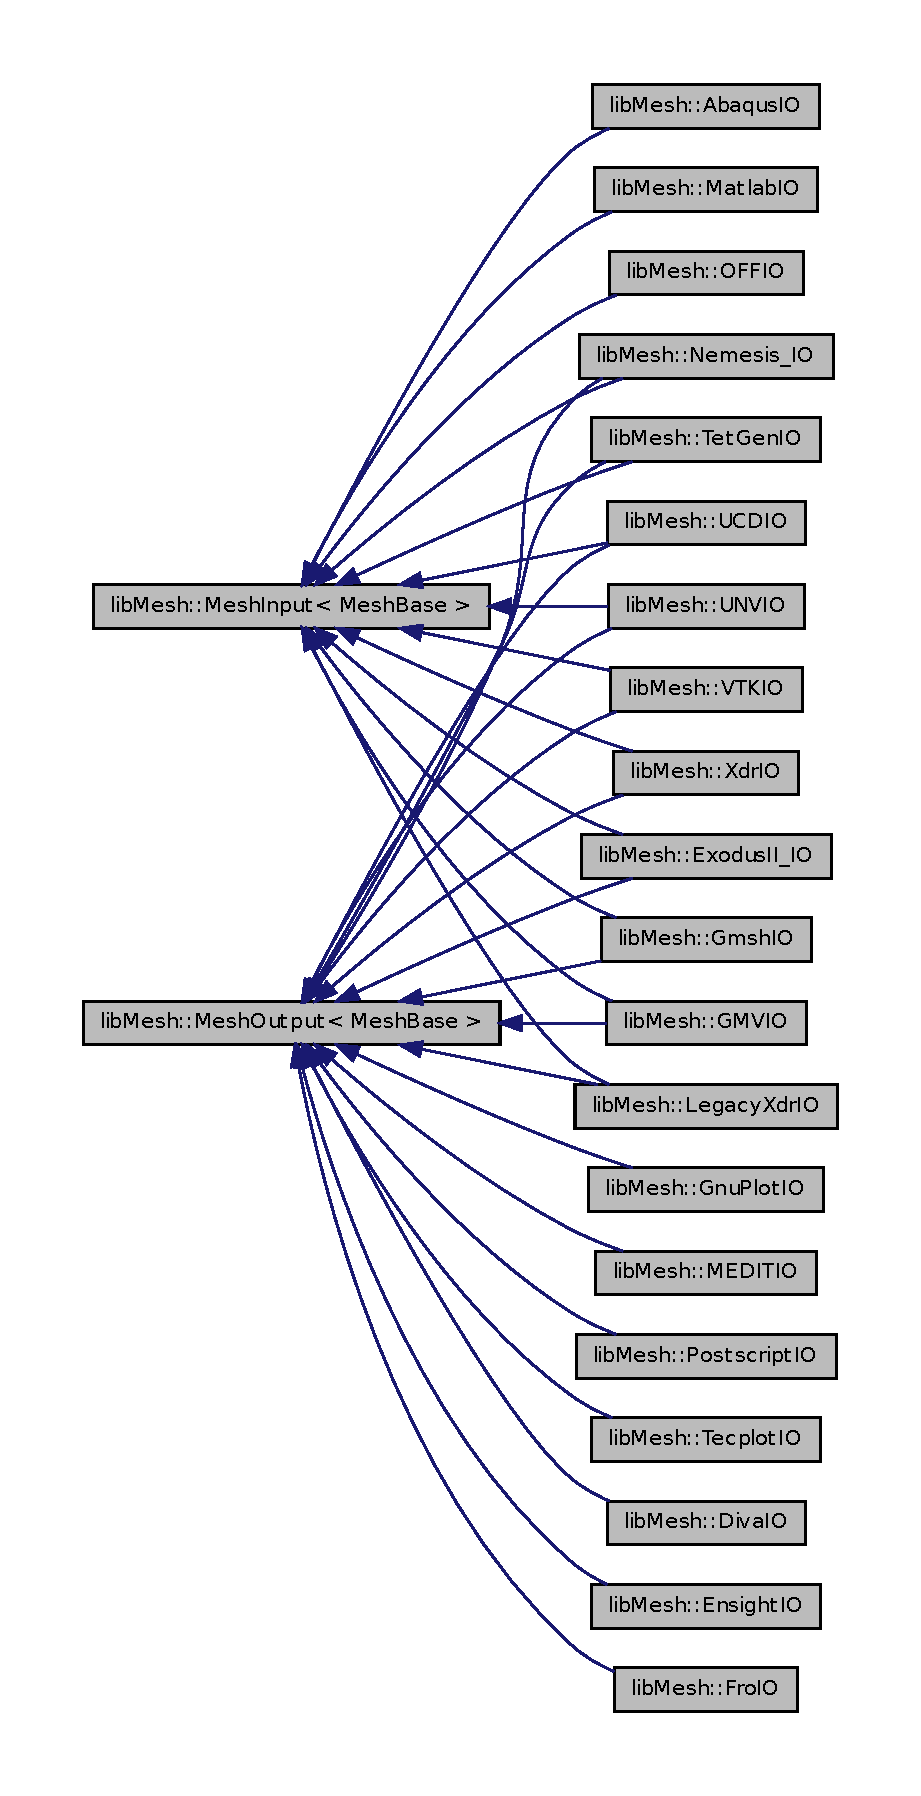
\includegraphics[height=0.9\textheight]{mesh_io}
  \end{center}
}


%%%%%%%%%%%%%%%%%%%%%%%%%%%%%%%%%%%%%%%%%%%%%%%%%
\frame
{
  \frametitle{Domain Partitioning}
  \begin{center}
    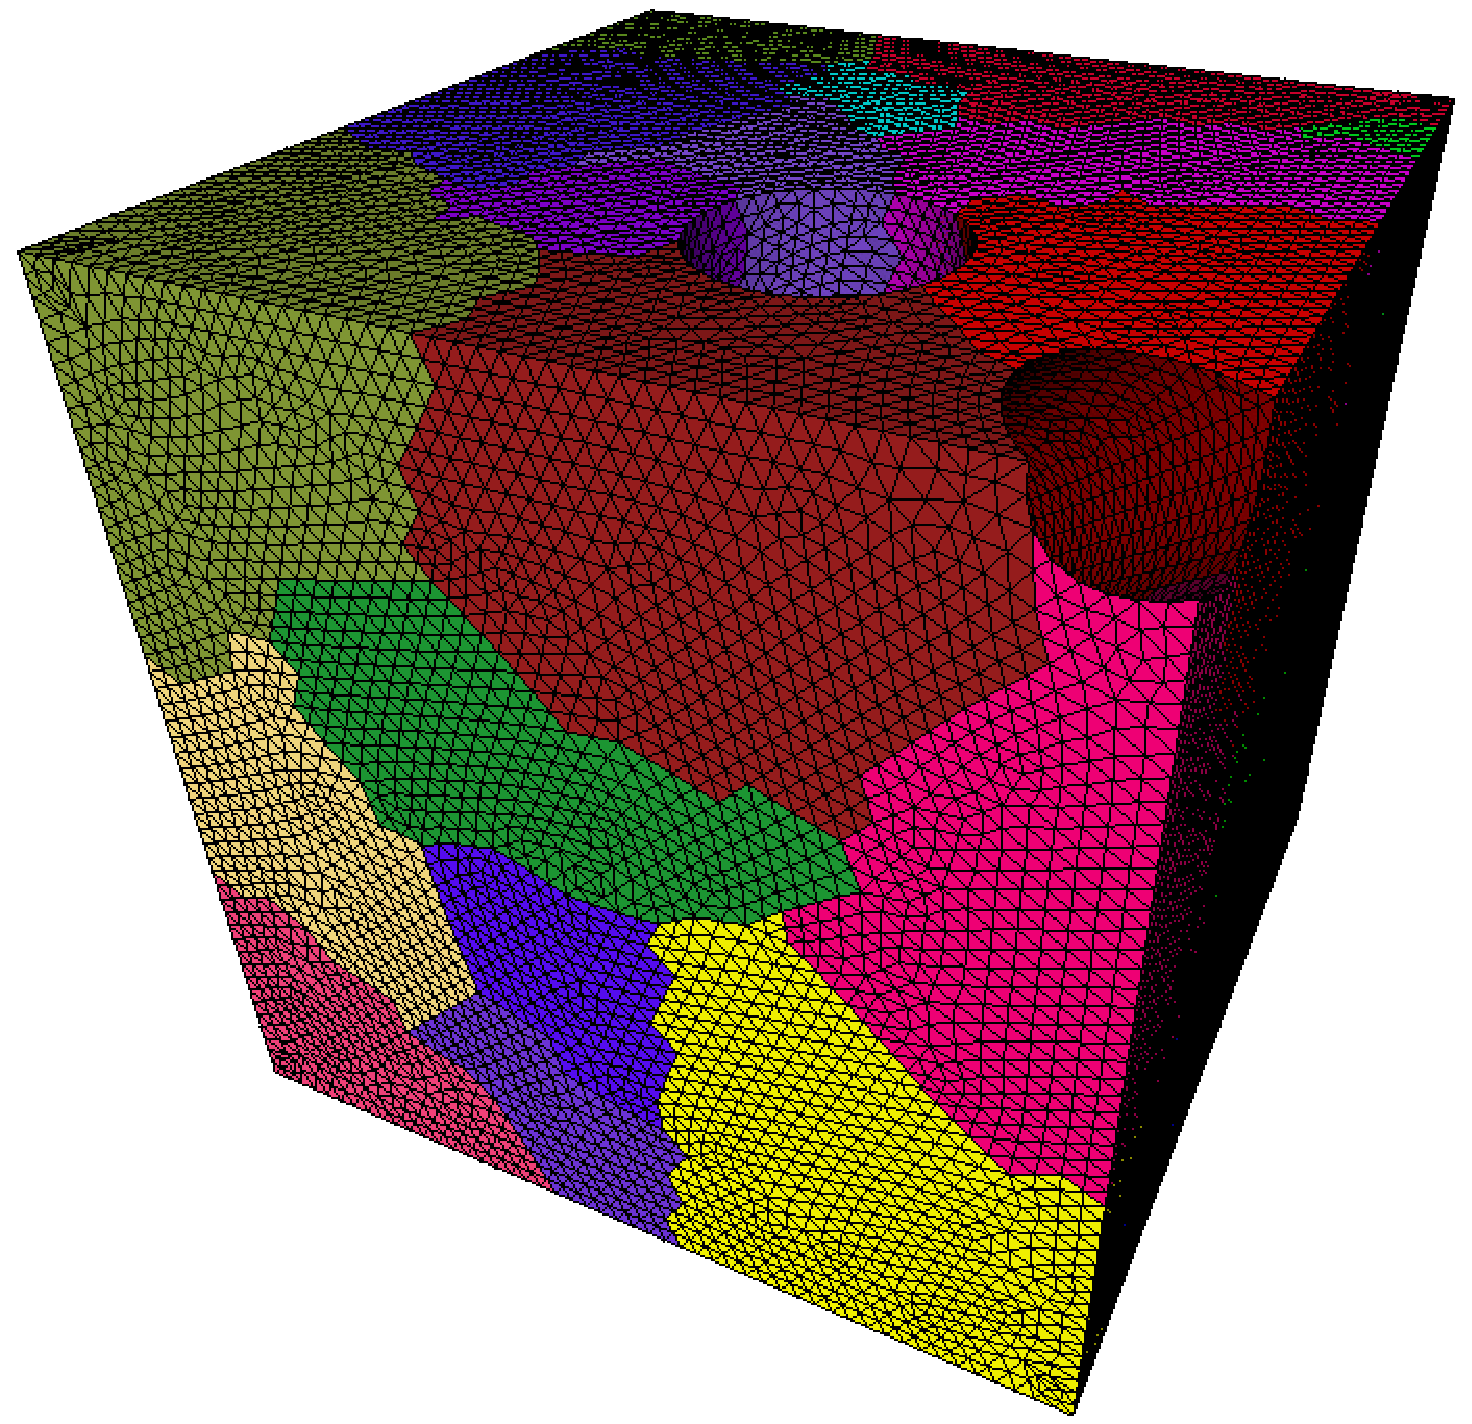
\includegraphics[width=.3\textwidth]{part_trans}
    %\\
    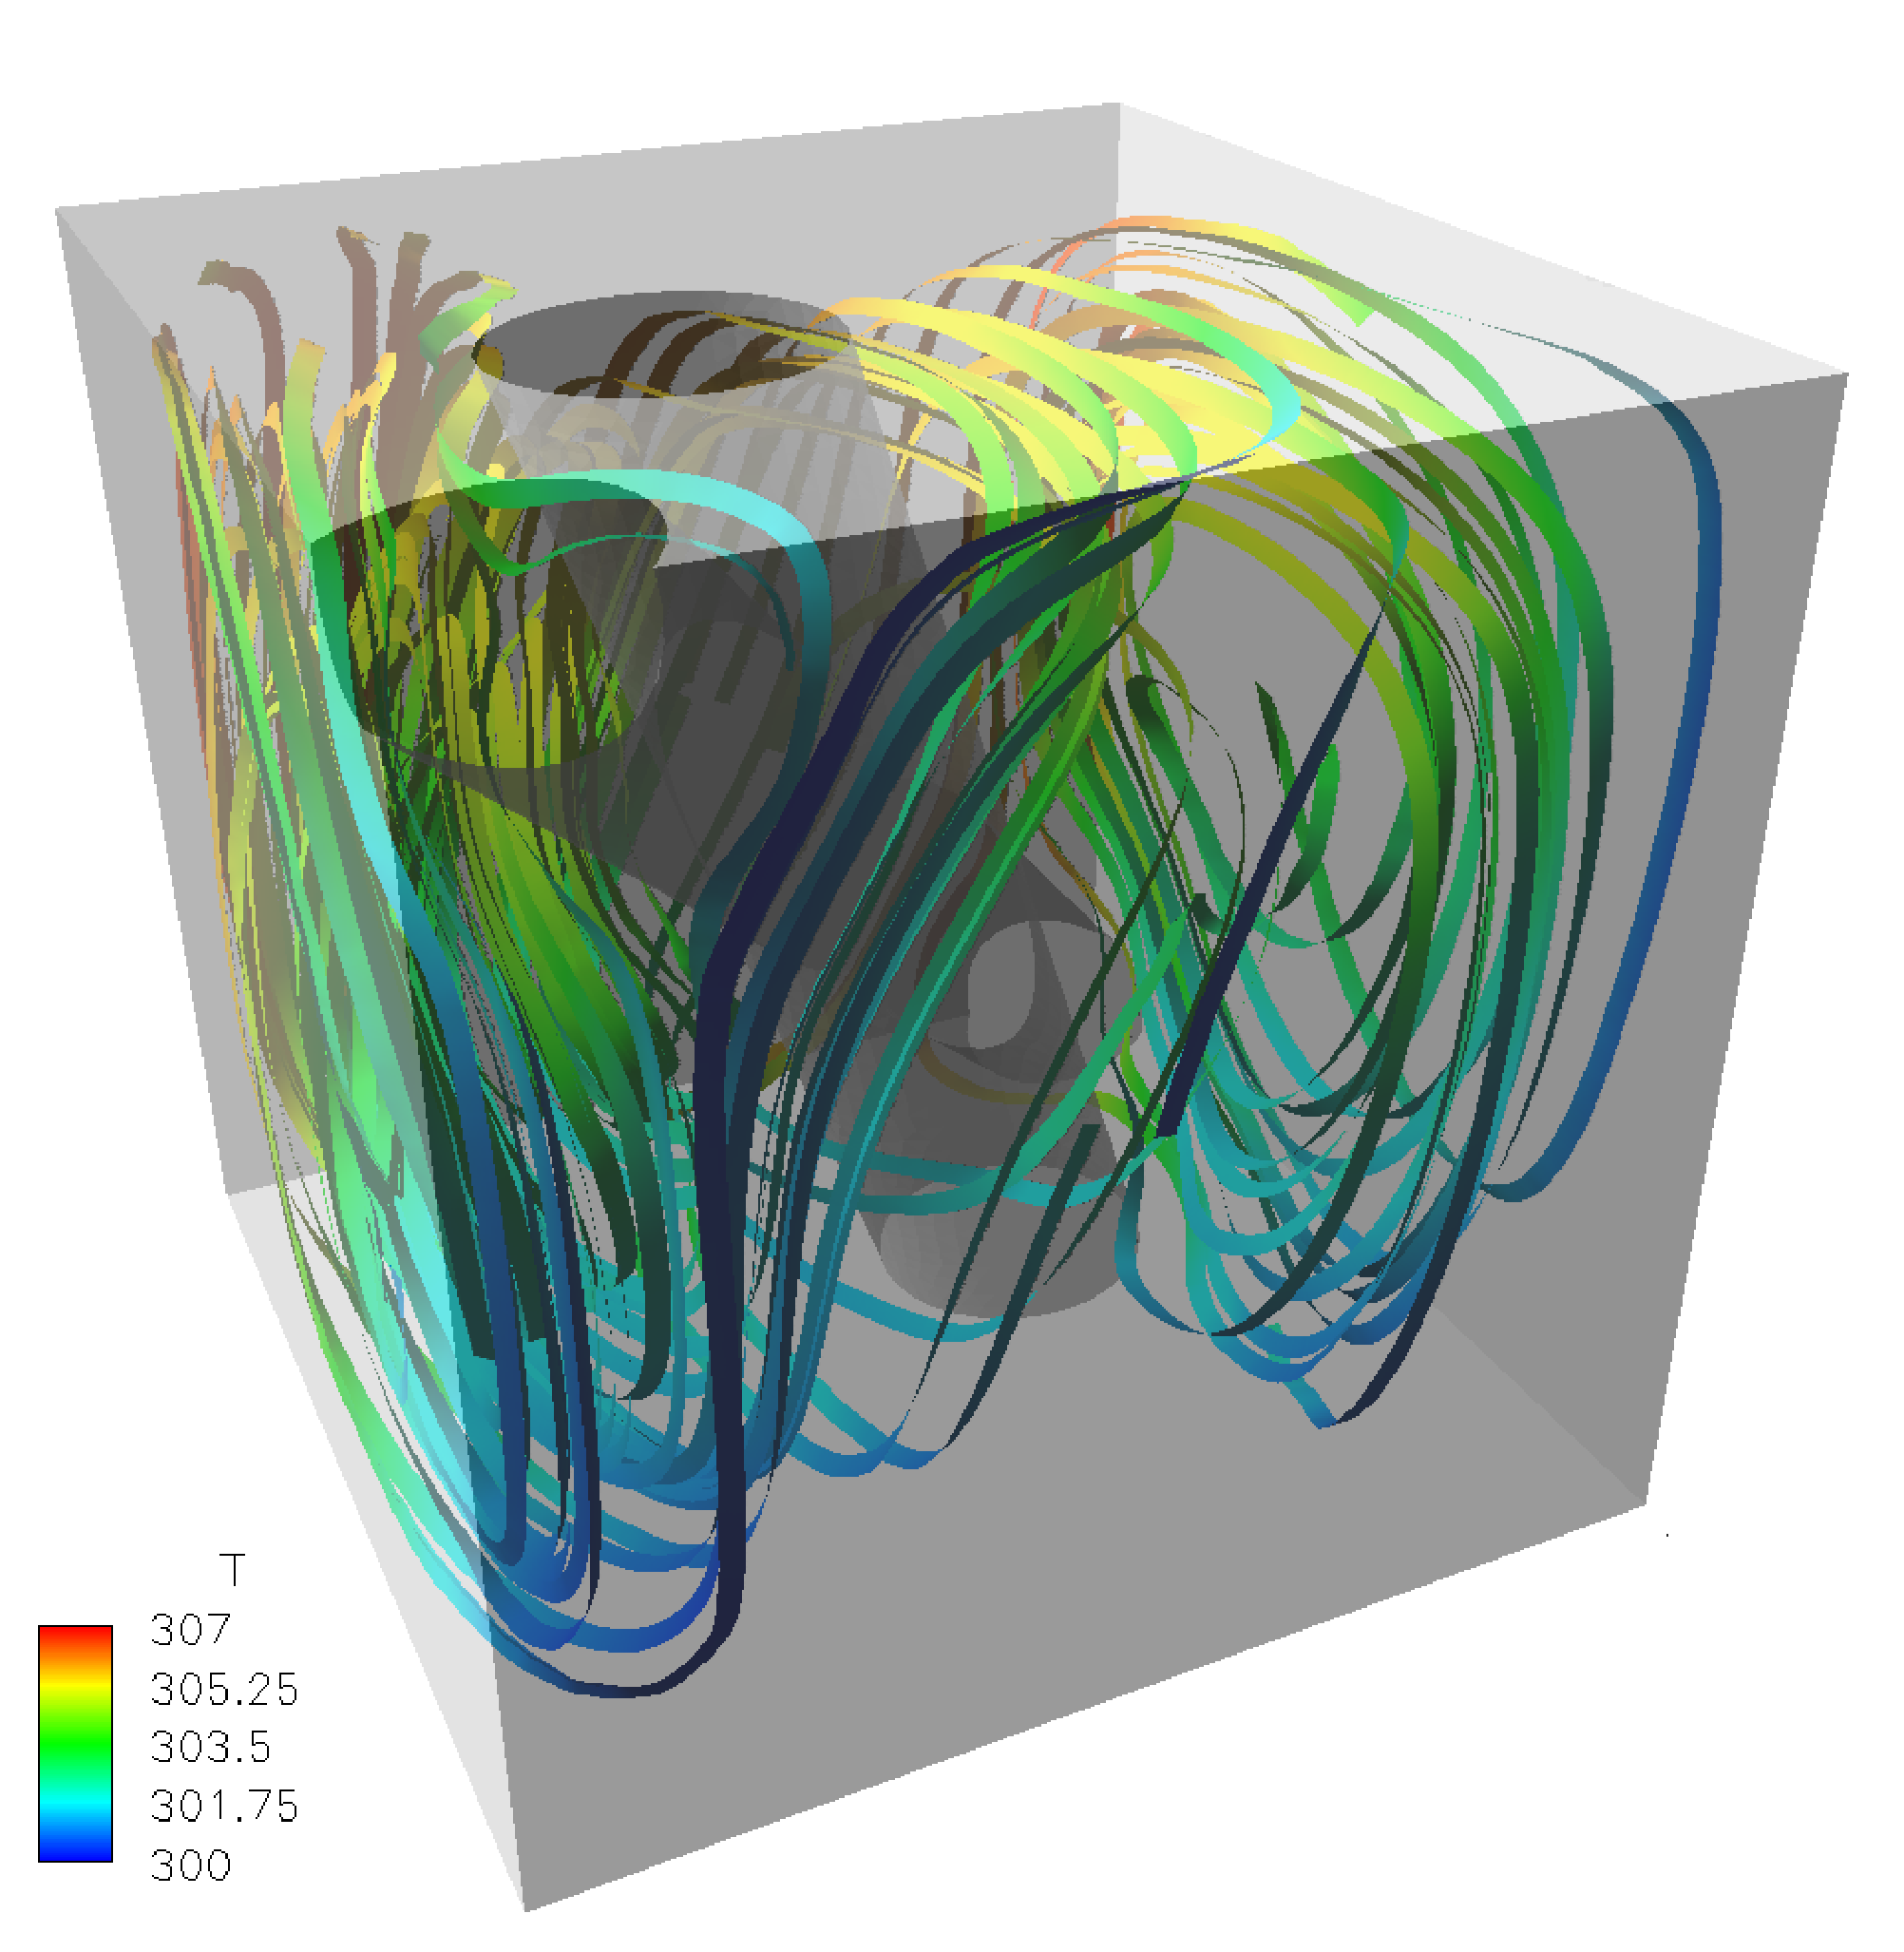
\includegraphics[width=.3\textwidth]{streamtraces}
  \end{center}  

  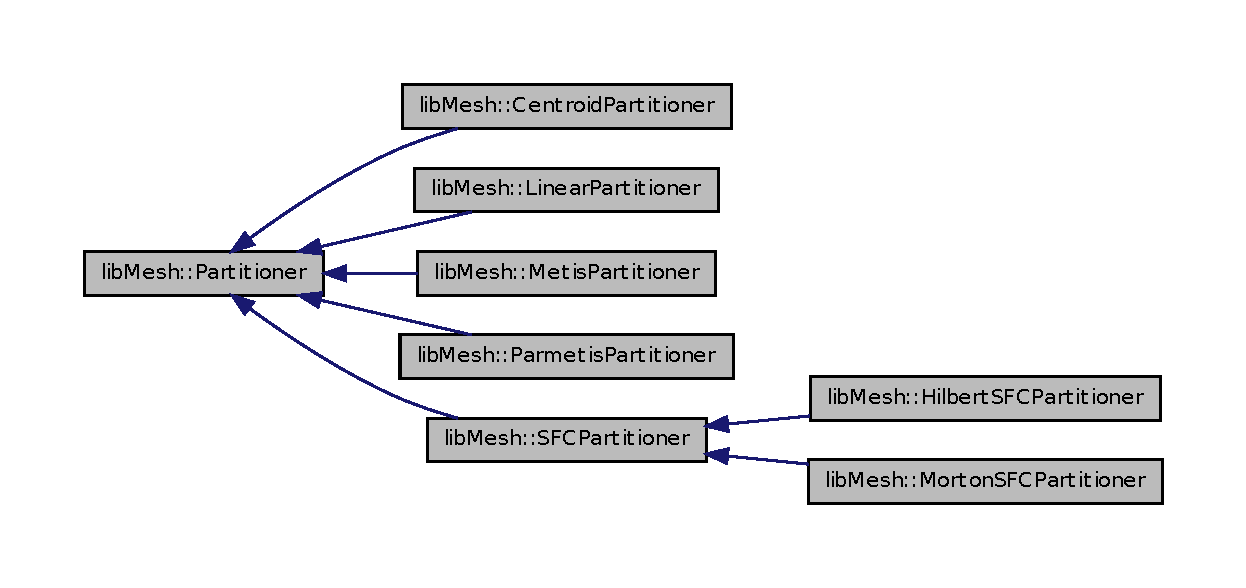
\includegraphics[width=.65\textwidth]{partitioner}
}


%%%%%%%%%%%%%%%%%%%%%%%%%%%%%%%%%%%%%%%%%%%%%%%%%
\begin{frame}
\frametitle{Mesh Data Structures}
\begin{columns}
\column{.6\textwidth}
\begin{center}
\includegraphics[width=.95\textwidth]{MeshUML}
\end{center}
\column{.4\textwidth}
%\begin{block}{}
\begin{itemize}
\item \texttt{MeshBase} gives node or element iterators, all vs active, global vs local
\item \texttt{ReplicatedMesh} or \texttt{DistributedMesh} manages synchronized or distributed data
\end{itemize}

\includegraphics[width=.75\textwidth]{ParallelMesh3}
%\end{block}
\end{columns}

\end{frame}



%%%%%%%%%%%%%%%%%%%%%%%%%%%%%%%%%%%%%%%%%%%%%%%%%
\frame
{
  \frametitle{Discretization: Finite Elements}
  \begin{center}
    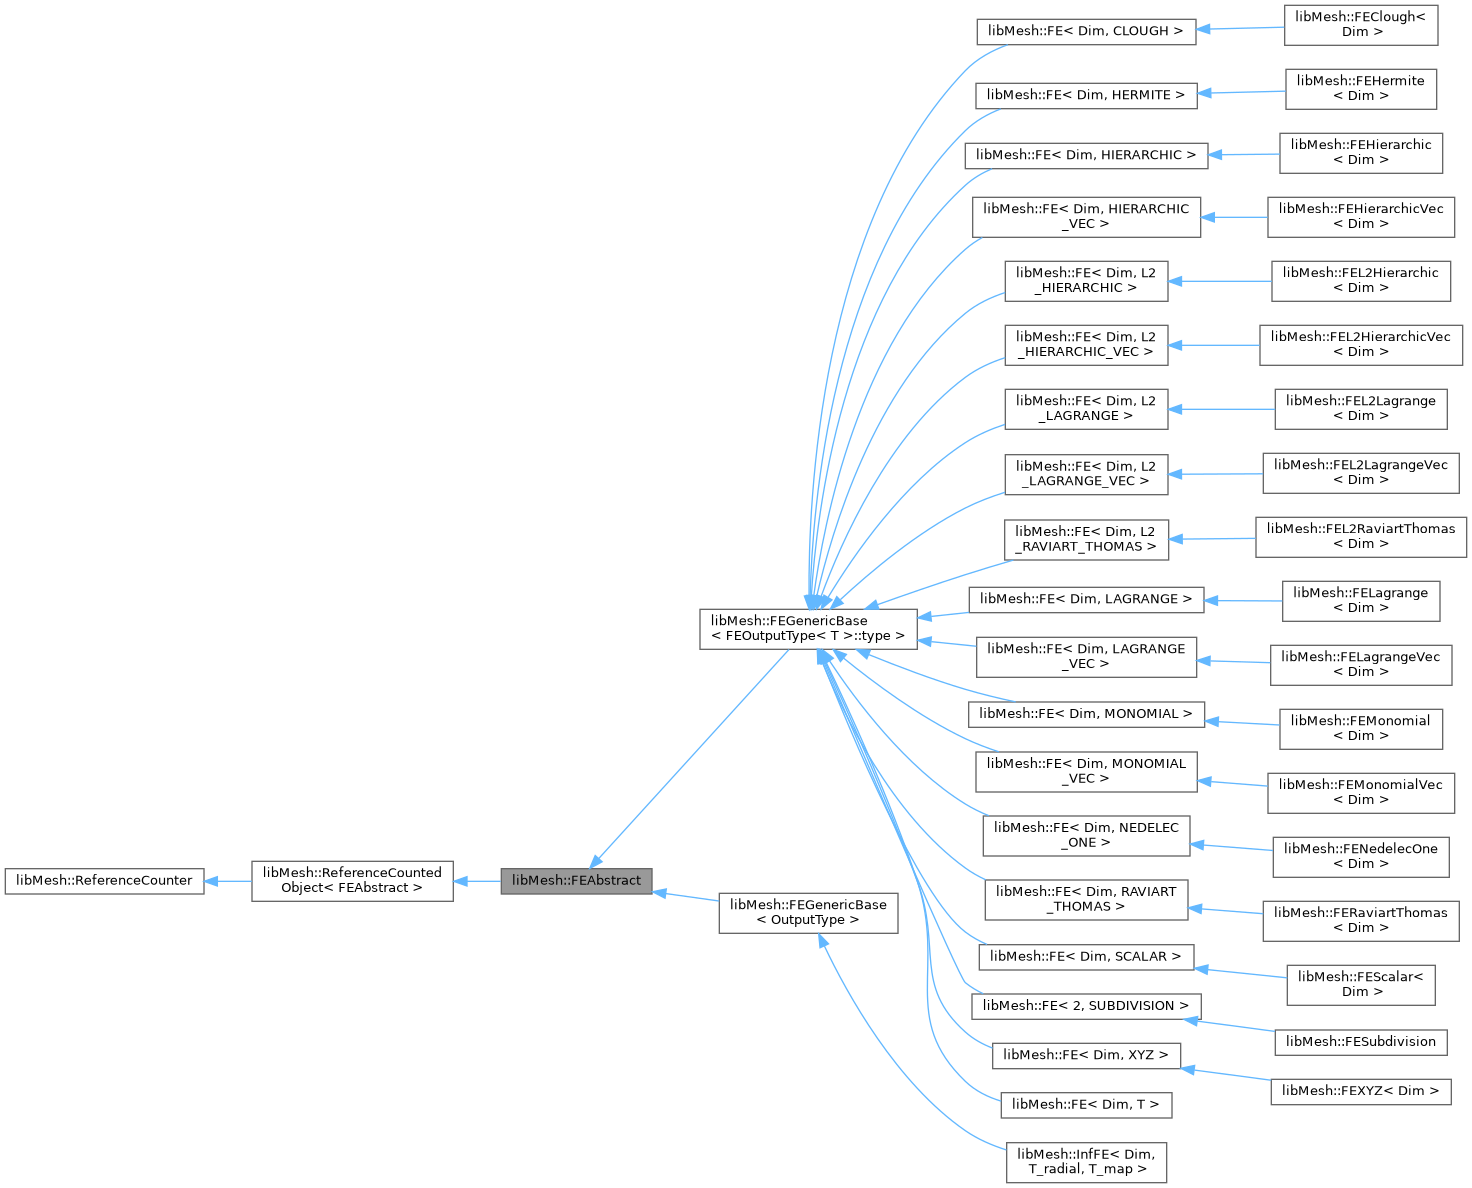
\includegraphics[width=0.9\textwidth,trim=7.4in 0 0 0,clip]{classlibMesh_1_1FEAbstract__inherit__graph}
  \end{center}
}      



%%%%%%%%%%%%%%%%%%%%%%%%%%%%%%%%%%%%%%%%%%%%%%%%%
\frame
{
  \frametitle{Algorithms: Error Estimation}
  \begin{center}
    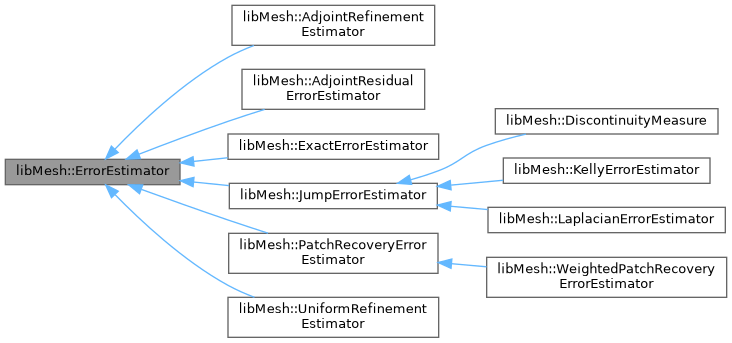
\includegraphics[width=\textwidth]{classlibMesh_1_1ErrorEstimator__inherit__graph}
  \end{center}
}



\section{\libMesh{} Core Classes}

%%%%%%%%%%%%%%%%%%%%%%%%%%%%%%%%%%%%%
\subsection{The Mesh Class}

\begin{frame}
  \frametitle{Operations on Objects in the \texttt{Mesh}}
  \begin{block}{}
    \begin{itemize}
    \item From a \texttt{Mesh} it is trivial to access ranges of objects of interest through \emph{iterators}.
    \item Iterators are simply a mechanism for accessing a range of objects.
    \item \libMesh{} makes extensive use of \emph{predictated iterators} to access, for example,
      \begin{itemize}
        \item All elements in the mesh.
        \item The ``active'' elements in the mesh assigned to the local processor in a parallel simulation.
        \item The nodes in the mesh.
      \end{itemize}
  \end{itemize}
  \end{block}
\end{frame}

\begin{frame}[shrink]
  \frametitle{Mesh Ranges and Iterators}
  \lstinputlisting{snippets/active_elem_iterators.cxx}
\end{frame}

\begin{frame}[shrink]
  \frametitle{Mesh Ranges and Iterators}
  \lstinputlisting{snippets/node_iterators.cxx}
\end{frame}



%%%%%%%%%%%%%%%%%%%%%%%%%%%%%%%%%%%%%
\subsection{The EquationSystems Class}
\begin{frame}
  \frametitle{EquationSystems}
  \begin{block}{}
    \begin{itemize}
      \item A \texttt{Mesh} is a discrete representation of problem geometry.
      \item For each \texttt{Mesh}, there can be an
        \texttt{EquationSystems} object, representing one or more
        coupled systems of equations posed on the \texttt{Mesh}.
        \begin{itemize}
          \item There is at most one \texttt{EquationSystems} object per \texttt{Mesh}.
          \item The \texttt{EquationSystems} object can hold many \texttt{System} objects, each representing a logical system of equations.
        \end{itemize}
      \item High-level operations such as solution input/output
        typically operate at the \texttt{EquationSystems} level.
      \item Each \texttt{System} has a degree-of-freedom mapping
        \texttt{DofMap} that assigns any DoF indices to each
        \texttt{DofObject} (\texttt{Elem} or \texttt{Node})
    \end{itemize}
  \end{block}
\end{frame}

\begin{frame}[shrink]
  \frametitle{EquationSystems}
  \lstinputlisting{snippets/es.cxx}
\end{frame}




%%%%%%%%%%%%%%%%%%%%%%%%%%%%%%%%%%%%%
\subsection{The \texttt{Elem} and \texttt{Node} Classes}
\begin{frame}
  \frametitle{Elements and Nodes}
  \begin{block}{Elements}
    \begin{itemize}
      \item The \texttt{Elem} base class is the interface to any geometric element in \libMesh{}.
      \item An \texttt{Elem} is defined by \texttt{Node}s, Edges (2D, 3D) and Faces (3D).
      \item An \texttt{Elem} is also a \texttt{DofObject} with
        more metadata:
        \begin{itemize}
          \item Global ID.
          \item Processor ownership.
          \item Degree of freedom indexing data.
          \item ``Extra'' integers or data
        \end{itemize}
    \end{itemize}
  \end{block}
  \begin{block}{Nodes}
    \begin{itemize}
      \item A \texttt{Node} is a \texttt{DofObject} which is also a
        \texttt{Point}, defining a location in 1D/2D/3D
    \end{itemize}
  \end{block}

\end{frame}

\begin{frame}[shrink]
  \frametitle{Elements and Nodes}
  \lstinputlisting{snippets/elem.cxx}
\end{frame}


%\section{Weighted Residuals}
%\input{outline_currentsection}

\begin{frame}[<+->]
      %\frametitle{Weighted Residual Statement}
  \begin{itemize}
  \item {The point of departure in any FE analysis which uses \libMesh{} is
    the weighted residual statement
    %(sometimes referred to as simply ``the residual'' in
    %the documentation.)
    \begin{equation}
      \nonumber
      (F( u ), v) = 0 \hspace{.5in} \forall v \in \mathcal{V}
    \end{equation}
    }

  \item{ Or, more precisely, the weighted residual statement associated with the
    finite-dimensional space $\mathcal{V}^h \subset \mathcal{V}$
    \begin{equation}
      \nonumber
      (F( u^{\alert{h}} ), v^{\alert{h}}) = 0 \hspace{.5in} \forall v^{\alert{h}} \in \mathcal{V}^{\alert{h}}
  \end{equation}}

  \item{ Even stabilized formulations boil down to some semilinear
          form
    \begin{equation}
      \nonumber
      \Res( u^{\alert{h}}, v^{\alert{h}}) = 0 \hspace{.5in} \forall v^{\alert{h}} \in \mathcal{V}^{\alert{h}}
  \end{equation}}

  \end{itemize}
\end{frame}


\subsection*{Some Examples}    
\begin{frame}[t]
  %\frametitle{Some Examples}
    \begin{block}{
	\only<1-2>{Poisson Equation}
	\only<3-4>{Linear Convection-Diffusion}
	\only<5-6>{Stokes Flow}
      }

      \only<1-2>
      {
	\begin{equation}
	      \nonumber
	      -\Delta u  = f
	      \hspace{.25in} \in \hspace{.1in} \Omega  
	    \end{equation}
      }
      
      \only<3-4>
	  {
	    \begin{equation}
	      \nonumber
	      %\frac{\partial u}{\partial t}
	      -k\Delta u + \bv{b} \cdot \nabla u = f
	      \hspace{.25in} \in \hspace{.1in} \Omega  
	    \end{equation}
	  }

      \only<5-6>
      {
	\begin{equation}
	    \begin{array}{rcl}
	      \nonumber
	      %\frac{\partial \bv{u}}{\partial t} +
	      %\left(\bv{u} \cdot \nabla\right) \bv{u} +
	      \nabla p - \nu \Delta \bv{u}  &=& \bv{f}
	        \\
	      \nonumber
	      \nabla \cdot \bv{u} &=& 0
	    \end{array}  \hspace{.25in}  \in \hspace{.1in} \Omega
	\end{equation}
      }

      
\end{block}
    %\pause

    \only<2,4,6>
    {
    \begin{block}{Weighted Residual Statement}
    }
      \only<2>
      {
      \begin{eqnarray}
	\nonumber
	(F( u ), v) := %\hspace{3in} \\  \nonumber
	\int_{\Omega}  \left[ \nabla u \cdot \nabla v - fv \right] dx \\ \nonumber
	+ \int_{\partial \Omega_N} \left(\nabla u \cdot \bv{n}\right) v \;ds
      \end{eqnarray}
%%       $^{\ast}$ We have employed the divergence theorem to obtain the weighted residual statement.
%%       In general this procedure gives rise to boundary terms which for simplicity we do not discuss
%%       in detail.
      }
      
    \only<4>
    {
      \begin{eqnarray}
	\nonumber
	(F( u ), v) := 
	\int_{\Omega} \left[
	  %\tfrac{\partial u}{\partial t}v  +
	  k\nabla u \cdot \nabla v + (\bv{b} \cdot \nabla u) v - fv \right] dx \\ \nonumber
	+ \int_{\partial \Omega_N} k\left(\nabla u \cdot \bv{n}\right) v \;ds
      \end{eqnarray}
    }

    \only<6>
    {
      \vspace{-.2in}
      \begin{eqnarray}
	\nonumber
	u := \left[\bv{u}, p\right]
	\hspace{.1in},\hspace{.1in}
	v := \left[\bv{v}, q\right]
      \end{eqnarray}
      \vspace{-.25in}
	\begin{eqnarray}
	  \nonumber
	(F( u ), v) := %\hspace{3in} \\ \nonumber
	\int_{\Omega} \left[
	  %\left( \tfrac{\partial \bv{u}}{\partial t}	  +
	  %\left( \bv{u} \cdot \nabla  \right)\bv{u}
	  %\right)
	  %\cdot \bv{v}
	- p\left(\nabla \cdot \bv{v}\right) 
	+ \nu \nabla \bv{u} \colon\!\! \nabla \bv{v} - \bv{f}\cdot \bv{v} \; \right. \\ \nonumber
	+ \left.\left( \nabla \cdot \bv{u} \right) q \right] dx
	+ \int_{\partial \Omega_N} \left(\nu \nabla \bv{u} -p\bv{I}\right)  \bv{n} \cdot \bv{v} \;ds %\hspace{1in}	
      \end{eqnarray}
    }
\only<2,4,6>
{
    \end{block}
 }     
\end{frame} 



%\subsection*{Approximate Problem}
\begin{frame}%[<+->]
  %\frametitle{Weighted Residual Statement}
  \begin{itemize}

    %%   \item{In each of the examples, the weighted residual statement is obtained by
    %%     multiplying the PDE by a test function $v$, integrating over the domain $\Omega$,
    %%     and applying the divergence theorem.}

    %%   \item{Since $v=0$ on $\partial \Omega_D$ (essential data) the boundary integrals
    %%     are over $\partial \Omega_N$ only.}

    %%   \item{There are simple and efficient techniques (e.g.\ penalty method) for
    %%     enforcing the Dirichlet conditions.}

  \item{To obtain the approximate problem, we simply
    replace $u \leftarrow u^h$, $v \leftarrow v^h$, and $\Omega \leftarrow \Omega^h$
    in the weighted residual
    statement.}
    
  \end{itemize}
\end{frame}

%\subsection{Poisson Equation}
%\input{outline_currentsection}

\subsection*{Weighted Residual Statement}
\begin{frame}%[<+->]
  %\frametitle{Poisson Equation}
  \begin{itemize}
  \item {For simplicity we start with the weighted
    residual statement arising from the Poisson equation,
    with $\partial \Omega_N = \emptyset$, 
    \begin{eqnarray}
      \nonumber
      (F( u^h ), v^h) := \hspace{2.5in} \\  \nonumber
      \int_{\Omega^h}  \left[ \nabla u^h \cdot \nabla v^h - fv^h \right] dx %\\ \nonumber
      %+ \int_{\partial \Omega^h_N} u_N v^h \;ds
      =0 \hspace{.5in} \forall v^{h} \in \mathcal{V}^{h}
    \end{eqnarray}
  }
  \end{itemize}
\end{frame}

\subsection*{Element Integrals}
\begin{frame}%[c]
%  \frametitle{Poisson Equation}
  \begin{itemize}    
  \item{
%%     \only<1>
%% 	{
	  The integral over $\Omega^h$ \ldots
%%	}
	  \visible<2->
	  {
	    is written as
	    a sum of integrals over the $\alert{N_e}$ finite elements: % $\Omega_e^h$
	  }
  }
  \end{itemize}
	  
  %\begin{block}{}
    \begin{eqnarray}
	\nonumber
	%(F( u^h ), v^h) &:=& %\hspace{3in} \\  \nonumber
	0 &=&
	\phantom{\sum_{e=1}^{N_e}}
	\int_{\Omega^h}  \left[ \nabla u^h \cdot \nabla v^h - fv^h \right] dx
	\hspace{.2in} \forall v^{h} \in \mathcal{V}^{h}
	\\ \nonumber
	\visible<2>
	    {
	&=&\alert{\sum_{e=1}^{N_e}}
	      \int_{\alert{\Omega_e}}
	      \left[ \nabla u^h \cdot \nabla v^h - fv^h \right] dx
	      \hspace{.2in} \forall v^{h} \in \mathcal{V}^{h}
	      \\ \nonumber
	    }
%% 	    \visible<3>
%% 		{
%% 	&=&\alert{\sum_{e=1}^{N_e}}
%% 	      \underbrace{\int_{\alert{\Omega_e}}
%% 	      \left[ \nabla u^h \cdot \nabla v^h - fv^h \right] dx}_{\text{We must compute this}}
%% 	      \hspace{.2in} \forall v^{h} \in \mathcal{V}^{h}
%% 		}
      \end{eqnarray}
    %\end{block}
%%     \begin{eqnarray}
%%       \nonumber
%%       (F( u^h ), v^h) &=& \int_{\Omega^h} (\ldots) \\
%%       \nonumber
%%       &=& \sum_{e=1}^{N_e} \int_{\Omega_e}(\ldots)\hspace{.25in} \forall v^{h} \in \mathcal{V}^{h}
%%     \end{eqnarray}
    
%  \item{The $v^h$ typically have support over only a small subset of the elements.}
\end{frame}

\subsection*{Finite Element Basis Functions}
\begin{frame}
  % \frametitle{Weighted Residual Statement}
    \begin{columns}[t]
    \column{.5\textwidth}
    \begin{block}{}
%%       \only<1>
%%       {
%% 	To node $i$ we associate a basis function $\psi_i$ such that for any $v^h \in \mathcal{V}^h$
%% 	we have
%% 	\begin{equation}
%% 	  \nonumber
%% 	  v^h = \sum_{i=1}^{N_n} c_i \psi_i
%% 	\end{equation}
%% 	for some constants $c_i$.
%%       }

%%       \only<2>
%%       {
%% 	\begin{itemize}
%% 	  \item{The $\psi_i$ are non-zero only over the elements adjacent to node $i$.}
%% 	  \item{For example, $\psi_i$ could be the linear ``hat'' function.
%% 	    %with value 1
%% 	    %at node $i$ and zero at all other nodes.
%% 	  }
%% 	\end{itemize}
%%       }

%%       \only<3->
%%       {
	\begin{itemize}
	  \item{An element integral will have contributions only
	    from the global basis functions corresponding to its nodes.}
	  \item{We call these local basis functions $\phi_i$, $0 \leq i \leq N_s$.}
	\end{itemize}
%%      }
    \end{block}

%%       \visible<3->
%%       {
	    \begin{equation}
	      \nonumber
	      \left. v^h \right|_{\Omega_e} = \sum_{i=1}^{N_s} c_i \phi_i
	    \end{equation}
%%      }
      \visible<2>
      {
	    \begin{equation}
	      \nonumber
	      \alert{\int_{\Omega_e}} v^h \;\alert{dx}
	      = \sum_{i=1}^{N_s} c_i \alert{\int_{\Omega_e}}\phi_i \;\alert{dx}
	    \end{equation}

      }
%}
%  \end{itemize}
    \column{.5\textwidth}
    %\begin{block}{}
      \begin{center}
%% 	\only<1>
%% 	    {
%% 	      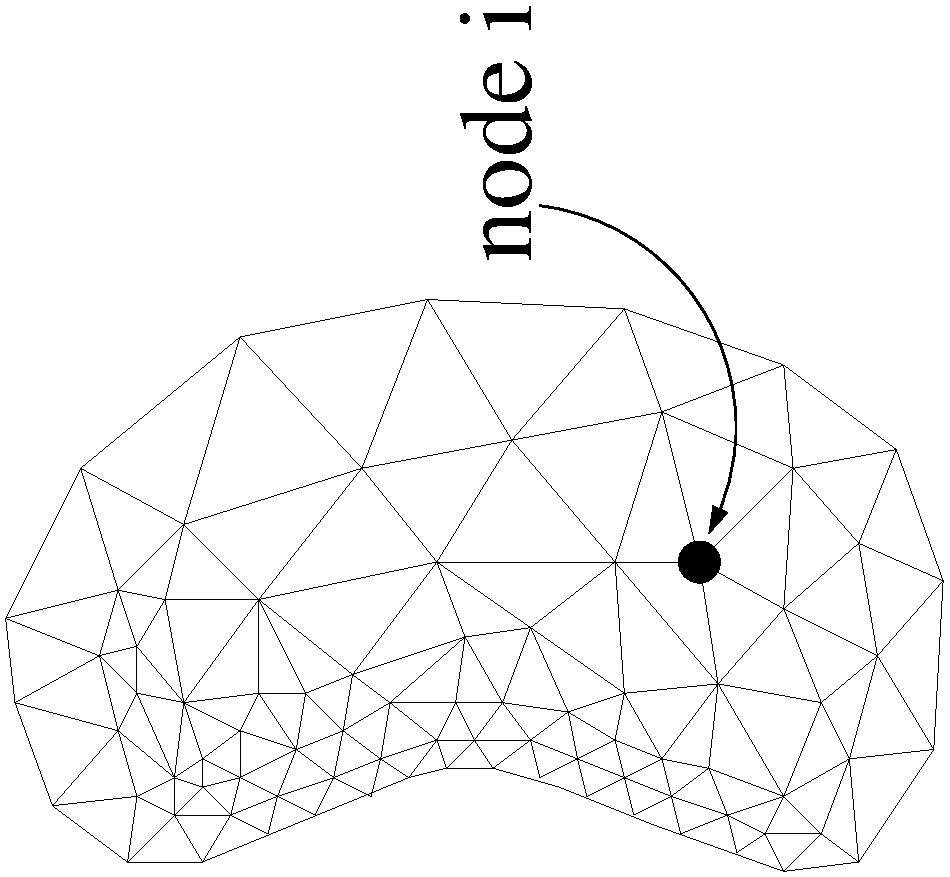
\includegraphics[width=2in,angle=-90]{node_i}
%% 	    }
%% 	\only<2>
%% 	    {
%% 	      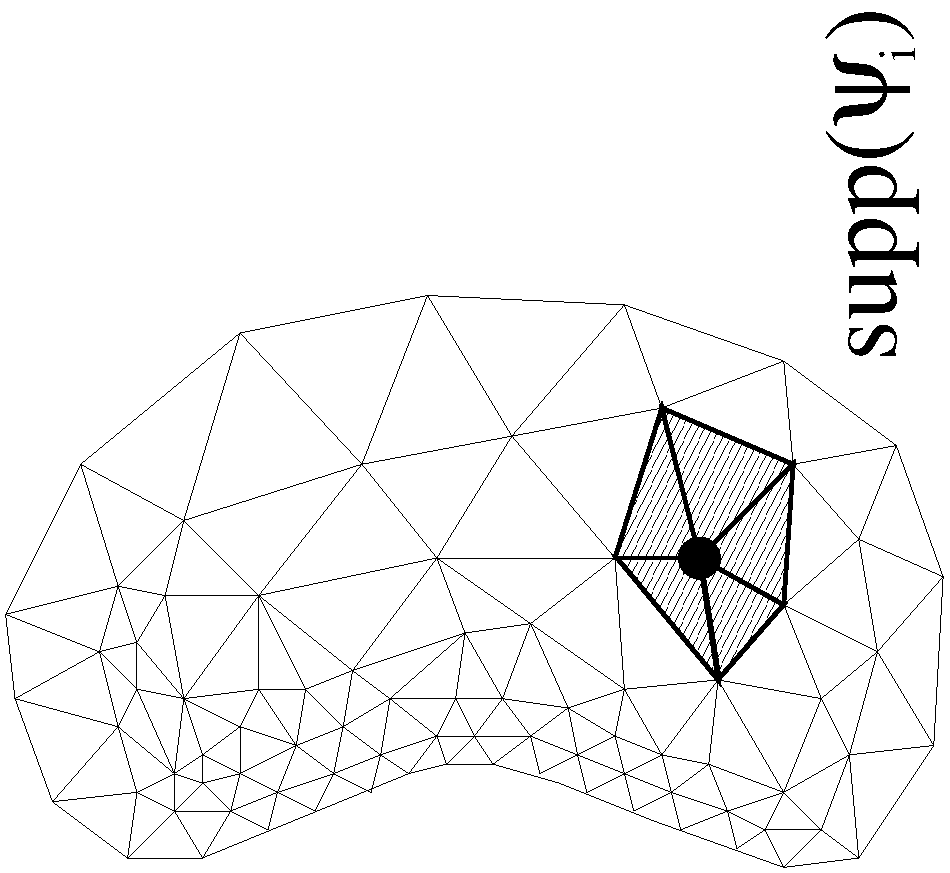
\includegraphics[width=2in,angle=-90]{phi_i}
%% 	    }
%% 	\only<3->
%% 	    {
	      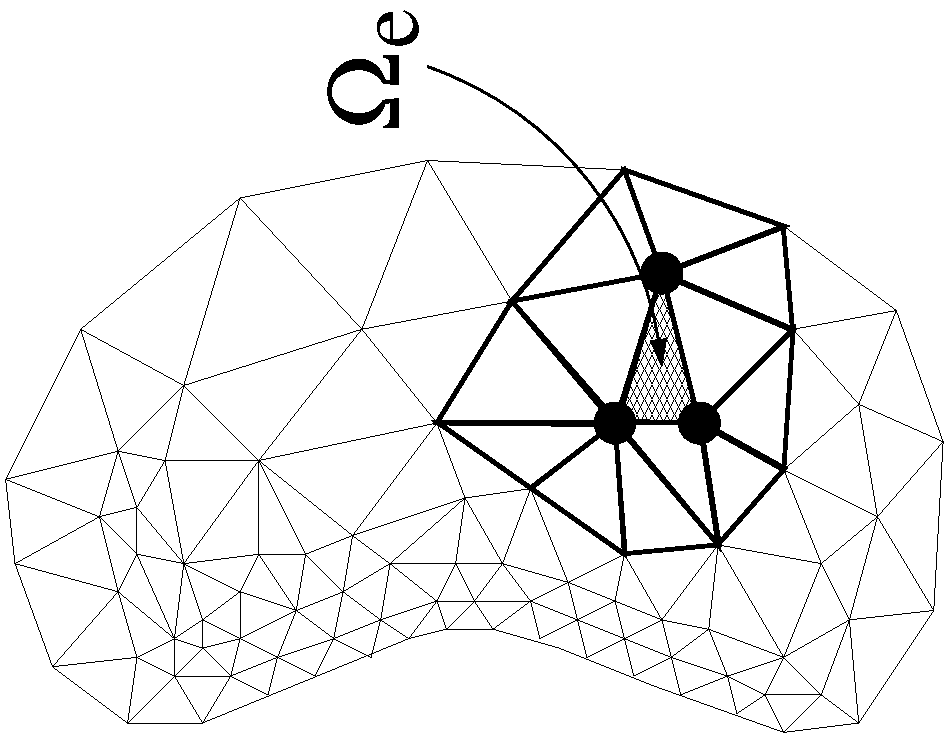
\includegraphics[width=2in,angle=-90]{phi_ijk}
%%	    }
      \end{center}
    \end{columns}
\end{frame}
    
\subsection*{Element Matrix and Load Vector}
\begin{frame}%[t]
%  \frametitle{Poisson Equation}
  \begin{itemize}    
    \visible<1->
	{
	\item
	  {
	    The element integrals \ldots
	    \begin{equation}
	      \nonumber
	      \int_{\Omega_e} \left[ \nabla u^h \cdot \nabla v^h - fv^h \right] dx
	    \end{equation}
	  }
	}

	
      \visible<2->
      {
	\item{
	  are written in terms of the local ``$\alert<2>{\phi_i}$'' basis functions
	  \begin{equation}
	    \nonumber
		\alert<2>{\sum_{j=1}^{N_s}}  \alert<2>{u_j}   \int_{\Omega_e}
		\nabla \alert<2>{\phi_j} \cdot \nabla \alert<2>{\phi_i} \;dx
		- \int_{\Omega_e}  f\alert<2>{\phi_i} \;dx
		\hspace{.15in},\hspace{.15in} i = 1,\ldots,N_s
	  \end{equation}
	}
      }
      \visible<3>
      {
	\item{
	  This can be expressed naturally in matrix notation as
	\begin{equation}
	  \nonumber
	  \bv{K^e} \bv{U^e} - \bv{F^e} 
	\end{equation}
	}
      }
  \end{itemize}
 \end{frame}



%% \frame%[t]
%%     {
%%   \frametitle{Poisson Equation}
%%   \begin{itemize}    
%%   \item
%%     {
%%       \visible<1->
%%       {
%% 	The element integrals \ldots
%%       }
%%       \visible<2->
%%       {
%% 	are written in terms of the local ``$\alert<2>{\phi_i}$'' basis functions \ldots
%%       }
%%       \visible<3>
%%       {
%% 	which can be expressed naturally in matrix notation.
%% 	%element ``stiffness matrix'' $\alert{\bv{K_e}}$
%% 	%and ``load vector'' $\alert{\bv{F_e}}$. 
%%       }
%%     }
%%   \end{itemize}
%%     \begin{eqnarray}
%%       %\begin{center}
%% 	\nonumber
%% 	%\begin{array}{c}
%% 	\int_{\Omega_e} \left[ \nabla u^h \cdot \nabla v^h - fv^h \right] dx
%% 	\hspace{.75in} \\ \nonumber
%% 	  \visible<2->
%% 	      {
%% 		\Downarrow \hspace{1.5in} \\ \nonumber
%% 		%
%% 		\alert<2>{\sum_{j=1}^{N_s}}  \alert<2>{u_j}   \int_{\Omega_e}
%% 		\nabla \alert<2>{\phi_j} \cdot \nabla \alert<2>{\phi_i} \;dx
%% 		- \int_{\Omega_e}  f\alert<2>{\phi_i} \;dx
%% 		\hspace{.15in},\hspace{.15in} i = 1,\ldots,N_s \\ \nonumber
%% 	      }
%% 	      \visible<3>
%% 	      {\Downarrow \hspace{1.5in} \\ \nonumber
%% 		%
%% 		\bv{K_e} \bv{U_e} - \bv{F_e} \hspace{1.25in}
%% 	      }
%% 	%\end{array}
%%       %\end{center}
%%     \end{eqnarray}
%%     }

\subsection*{Global Linear System}
\begin{frame}%[<+->]
  %  \frametitle{Poisson Equation}
  \begin{itemize}
    \visible<1->{
    \item{
      The entries of the element stiffness matrix are the integrals
      \begin{equation}
	\nonumber
	\bv{K}^e_{ij} := 
	\int_{\Omega_e}
	\nabla \phi_j \cdot \nabla \phi_i \;dx
      \end{equation}
    }
    }
    \visible<2->{
    \item{ While for the element right-hand side we have 
      \begin{equation}
	\nonumber
	\bv{F}^e_{i} := 
	\int_{\Omega_e} f \phi_i \;dx
      \end{equation}
    }
    }
    \visible<3>{
    \item{ The element stiffness matrices and right-hand sides can be ``assembled'' to 
      obtain the global system of equations
      \begin{equation}
	\nonumber
	\bv{K} \bv{U} = \bv{F}
      \end{equation}    
    }
    }
  \end{itemize}
\end{frame}

\subsection*{Reference Element Map}


\begin{frame}[t]
%  \frametitle{Poisson Equation}
  \begin{block}{}
    \begin{itemize}    
  \item{
    The integrals are performed on a ``reference'' element $\alert<1>{\hat{\Omega}_e}$
    }
  \end{itemize}
  \end{block}
  %\vspace{-.3in}
  %\begin{center}   %Note: \centering is what makes the tables ``wiggle'' during slide transitions
  %% Three separate tabular elements.  The first column is an empty, fixed-width column designed
  %% to center the table without using centering commands.
    \only<1>
    {
    \begin{tabular}{p{.125\textwidth}ccc} \\
      &
      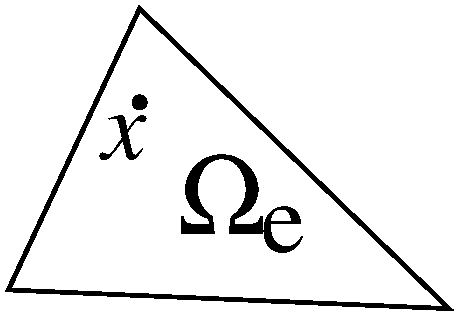
\includegraphics[width=.2\textwidth]{physical_element}&
      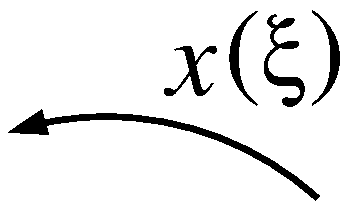
\includegraphics[width=.2\textwidth]{map}&
      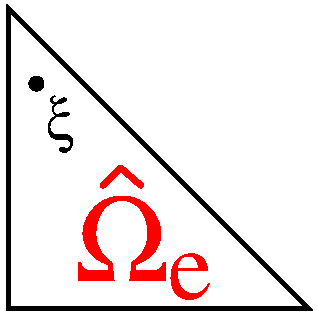
\includegraphics[width=.15\textwidth]{reference_element_red}
    \end{tabular}
    }
    %
    \only<2>
    {
    \begin{tabular}{p{.125\textwidth}ccc} \\ 
      &
      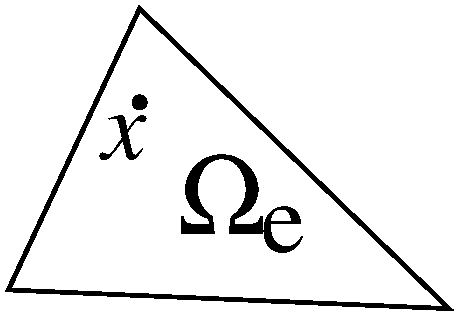
\includegraphics[width=.2\textwidth]{physical_element}&
      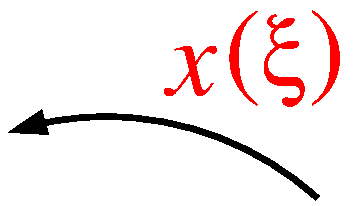
\includegraphics[width=.2\textwidth]{map_red}&
      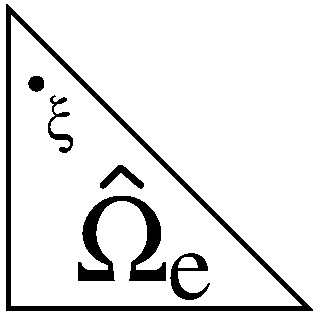
\includegraphics[width=.15\textwidth]{reference_element}
    \end{tabular}
    }
    %
    \only<3>
    {
    \begin{tabular}{p{.125\textwidth}ccc} \\ 
      &
      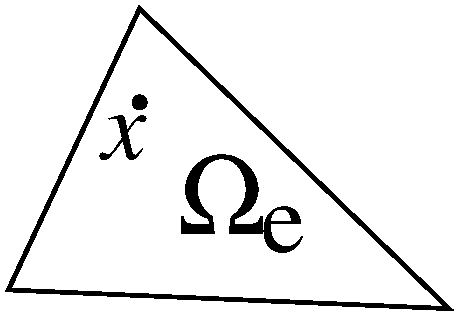
\includegraphics[width=.2\textwidth]{physical_element}&
      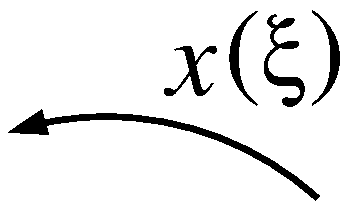
\includegraphics[width=.2\textwidth]{map}&
      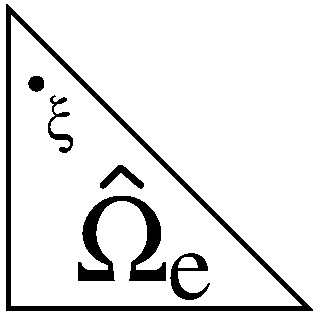
\includegraphics[width=.15\textwidth]{reference_element}
    \end{tabular}
    }
    
%%     %% All in one table
%%     \begin{tabular}{ccc} \\ 
%%     %\fbox{
%%       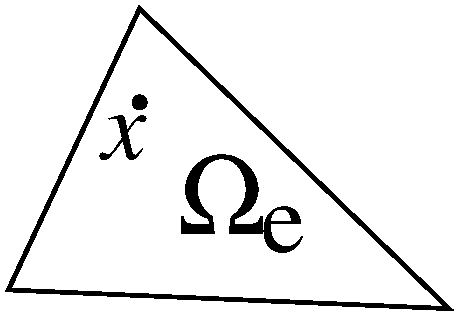
\includegraphics[width=.2\textwidth]{physical_element}
%%     %}
%%        &
%%   \only<1,3->
%%   {
%%        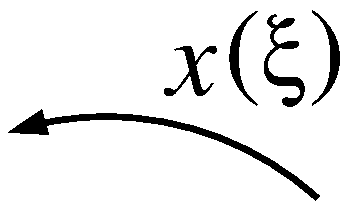
\includegraphics[width=.2\textwidth]{map}
%%   }
%%   \only<2>
%%   {
%%        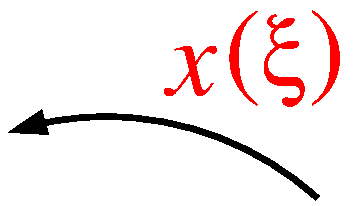
\includegraphics[width=.2\textwidth]{map_red}
%%   }
%%        &
%%   \only<1>
%%   {
%%        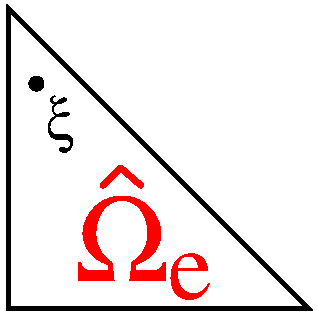
\includegraphics[width=.15\textwidth]{reference_element_red}
%%        }
%%   \only<2->
%%   {
%%        \includegraphics[width=.15\textwidth]{reference_element}
%%        }
%%      \end{tabular}
  %\end{center}


  \only<2>
      {
	\begin{block}{}
	\begin{itemize}    
	\item{
	  The Jacobian of the map $\alert{x(\xi)}$ is $\alert{J}$.
	}
	\end{itemize}
	\end{block}
	\begin{equation}
	  \nonumber
	  \bv{F}^e_{i} = \int_{\Omega_e} f \phi_i dx
	  =  \int_{\alert{\hat{\Omega}_e}}
	  f (\alert{x(\xi)}) \phi_i \alert{|J|} d\alert{\xi}
	\end{equation}
      }

\only<3>
{
  \begin{block}{}
  \begin{itemize}    
  \item{
    %The gradients are transformed
    Chain rule: 
    $\nabla 
    = J^{-1}\nabla_{\!\xi}
    := \alert{\hat{\nabla}_{\!\xi}}$
  }
  \end{itemize}
  \end{block}
  \begin{equation}
    \nonumber
    \bv{K}^e_{ij} =
    \int_{\Omega_e}
    \nabla \phi_j \cdot \nabla \phi_i \;dx =
    \int_{\hat{\Omega}_e}
    \alert{\hat{\nabla}_{\!\xi}} \phi_j \cdot
    \alert{\hat{\nabla}_{\!\xi}} \phi_i \;|J| d\xi
  \end{equation}
}
\end{frame}

\subsection*{Element Quadrature}
    
\begin{frame}[t]
%	\frametitle{Poisson Equation}
	\begin{block}{}
	\begin{itemize}    
	\item{
	  The integrals on the ``reference'' element are approximated via numerical
	  quadrature.
	}
	  \visible<2->
	      {
	      \item{The quadrature rule has $\alert{N_q}$ points
		``$\alert{\xi_q}$'' and weights ``$\alert{w_q}$''.}
	      }
	\end{itemize}
	\end{block}
\only<3>
{
	\begin{eqnarray}
	  \nonumber
%	  \only<3-4>
%	      {
		\bv{F}^e_{i} &=&
		\int_{\hat{\Omega}_e} f \phi_i |J| d\xi
		\\ \nonumber
%	      }
%	      \only<4>
%		  {
		    &\approx&
		    \alert{\sum_{q=1}^{N_q}}
		    f(x(\alert{\xi_q})) \phi_i(\alert{\xi_q})
		    |J(\alert{\xi_q})| \alert{w_q}
%		  }
	\end{eqnarray}
}

\only<4>
{
	\begin{eqnarray}
	  \nonumber
%	  \only<5-6>
%	      {
		\bv{K}^e_{ij} &=&
		\int_{\hat{\Omega}_e}
		\hat{\nabla}_{\!\xi}\phi_j \cdot
		\hat{\nabla}_{\!\xi}\phi_i \;|J| d\xi
		\\ \nonumber
%	      }
%	      \only<6>
%		  {
		    &\approx&
		    \alert{\sum_{q=1}^{N_q}}
		    \hat{\nabla}_{\!\xi} \phi_j(\alert{\xi_q}) \cdot
		    \hat{\nabla}_{\!\xi} \phi_i(\alert{\xi_q})
		    |J(\alert{\xi_q})| \alert{w_q}
%		  }
	\end{eqnarray}
}
\end{frame}

\subsection*{\libMesh{} Quadrature Point Data}
\begin{frame}[t]
%	\frametitle{Poisson Equation}
	\begin{block}{}
	\begin{itemize}    
	\item{ \libMesh{} provides the following variables at
	  each quadrature point $q$
	}
%% 	\item{``\texttt{JxW[q]}'' = $|J(\xi_q)| w_q$
%% 	  %the scalar value of the element Jacobian map times
%% 	  %the quadrature rule weight
%% 	}
	\end{itemize}
	\end{block}
	
	\begin{center}
	  \renewcommand{\arraystretch}{1.3}
	\begin{tabular}{|l|l|l|} \hline
	  \textbf{Code} & \textbf{Math} & \textbf{Description} \\ \hline
	  \texttt{JxW[q]}
	  & $|J(\xi_q)| w_q$
	  & Jacobian times weight
	  \\ \hline
	  \texttt{phi[i][q]}
	  & $\phi_i(\xi_{q})$
	  & value of $i^{th}$ shape fn.\
	  \\ \hline
	  \texttt{dphi[i][q]}
	  & $\hat{\nabla}_{\!\xi} \phi_i (\xi_q)$
	  & value of $i^{th}$ shape fn.\ gradient
	  \\ \hline
	  \texttt{d2phi[i][q]}
	  & $\hat{\nabla}^2_{\!\xi} \phi_i (\xi_q)$
	  & value of $i^{th}$ shape fn.\ Hessian
	  \\ \hline
	  \texttt{xyz[q]}
	  & $x(\xi_q)$
	  & location of $\xi_q$ in physical space
	  \\ \hline
	  \end{tabular}
	\end{center}
	  
%      } %end frame
\end{frame}

\subsection*{Matrix Assembly Loops}
\begin{frame}[fragile,t]  
%  \frametitle{Poisson Equation}
	\begin{block}{}
	  \begin{itemize}    
	  \item{ The \libMesh{} representation of the matrix and
	    rhs assembly is similar to the mathematical statements.
	  }
	  \end{itemize}
	\end{block}
\small
\begin{semiverbatim}
for (q=0; q<Nq; ++q) 
  for (i=0; i<Ns; ++i) \{
    \alert<2>{Fe(i)   += \alert<3>{JxW[q]}*\alert<4>{f(xyz[q])}*\alert<5>{phi[i][q]};}
    
    for (j=0; j<Ns; ++j)
      \alert<6>{Ke(i,j) += \alert<7>{JxW[q]}*(\alert<8>{dphi[j][q]*dphi[i][q]});}
  \}
\end{semiverbatim}
\only<2-5>
{
  \begin{equation}
    \nonumber
    \bv{F}^e_{i} = 
    \sum_{q=1}^{N_q}
    \alert<4>{f(x(\xi_q))}
    \alert<5>{\phi_i(\xi_q)}
    \alert<3>{|J(\xi_q)| w_q}
  \end{equation}
}
\only<6->
{
  \begin{equation}
  \nonumber
  \bv{K}^e_{ij} =
  \sum_{q=1}^{N_q}
  \alert<8>{
    \hat{\nabla}_{\!\xi} \phi_j(\xi_q) \cdot
    \hat{\nabla}_{\!\xi} \phi_i(\xi_q)
    }
  \alert<7>{|J(\xi_q)| w_q}
  \end{equation}
}
\end{frame}

      

%\subsection{Other Examples}
%\input{outline_currentsection}


\subsection*{Convection-Diffusion Equation}
\begin{frame}[fragile]  
  \begin{block}{}
    \begin{itemize}    
    \item{The matrix assembly routine for the linear convection-diffusion equation,
      \begin{equation}
	\nonumber
	-\alert<2>{k}\Delta u + \alert<3>{\bv{b} \cdot \nabla u} = f
      \end{equation}
    }
    \end{itemize}
  \end{block}
  \small
  \begin{semiverbatim}
for (q=0; q<Nq; ++q) 
  for (i=0; i<Ns; ++i) \{
    Fe(i)   += JxW[q]*f(xyz[q])*phi[i][q];
    
    for (j=0; j<Ns; ++j)
      Ke(i,j) += JxW[q]*(\alert<2>{k}*(dphi[j][q]*dphi[i][q]) 
                       +(\alert<3>{b*dphi[j][q]})*phi[i][q]);
  \}
  \end{semiverbatim}
\end{frame}

\subsection*{Stokes Flow}
\begin{frame}[t]  
  \begin{block}{}
    \begin{itemize}    
    \item{For multi-variable systems like Stokes flow,
      \begin{equation}
	\begin{array}{rcl}
	  \nonumber
	  %\frac{\partial \bv{u}}{\partial t} +
	  %\left(\bv{u} \cdot \nabla\right) \bv{u} +
	  \nabla p - \nu \Delta \bv{u}  &=& \bv{f}
	  \\
	  \nonumber
	  \nabla \cdot \bv{u} &=& 0
	\end{array}  \hspace{.25in}  \in \hspace{.1in} \Omega \subset \mathbb{R}^2
      \end{equation}
    }
\vspace{-.25in}
      
    \item{The element stiffness matrix concept can extended to include sub-matrices
      \begin{eqnarray}
	\nonumber
	\label{eqn:Ke_stokes}
	\left[
	  \begin{array}{cc|c}
	    \alert<2>{K^e_{u_1 u_1}}   & K^e_{u_1 u_2}             &  K^e_{u_1 p}        \\
	    K^e_{u_2 u_1}              & \alert<3>{K^e_{u_2 u_2}}  &  K^e_{u_2 p} \\ \hline
	    K^e_{p u_1}                & \alert<4>{K^e_{p u_2}}    &  K^e_{p p}      \\
	  \end{array}
	  \right]
	\left[
  \begin{array}{c}
    U^e_{u_1} \\
    U^e_{u_2}\\ \hline
    U^e_{p}
  \end{array}
  \right]-
\left[
  \begin{array}{c}
    \alert<6>{F^e_{u_{1}}} \\
    \alert<7>{F^e_{u_{2}}} \\ \hline
    F^e_{p}
  \end{array}
  \right]
      \end{eqnarray}
    }


      \item
	{
	  \only<1-4>	      {We have an array of submatrices:}
	      \only<1>	      {\texttt{Ke[ ][ ]}}
	      \only<2>	      {\hspace{-0.05in}\texttt{Ke[\alert<2>{0}][\alert<2>{0}]}}
	      \only<3>	      {\hspace{-0.1in}\texttt{Ke[\alert<3>{1}][\alert<3>{1}]}}
	      \only<4>        {\hspace{-0.15in}\texttt{Ke[\alert<4>{2}][\alert<4>{1}]}}

      \only<5->          { 	  And an array of right-hand sides: }
 	\only<5> {\texttt{Fe[]}.}
	\only<6> {\hspace{-0.05in}\texttt{Fe[\alert{0}]}.}
	\only<7> {\hspace{-0.1in}\texttt{Fe[\alert{1}]}.}
	}

	
%%       \only<1>
%% 	  {
%% 	  \item{
%% 	    We have an array of submatrices
%% 	    \texttt{Ke[ ][ ]}.
%% 	  }
%% 	  }

%% 	  \only<2>
%% 	  {
%% 	  \item{
%% 	    We have an array of submatrices
%% 	    \texttt{Ke[\alert<2>{1}][\alert<2>{1}]}.
%% 	  }
%% 	  } 
%%           \only<3>
%%           {
%%  	  \item{
%%  	    In this case, we have an array of submatrices
%%  	    \texttt{Ke[\alert<3>{2}][\alert<3>{2}]}.
%%  	  }
%% 	  }
%%           \only<4>
%%           {
%%  	  \item{
%%  	    In this case, we have an array of submatrices
%%  	    \texttt{Ke[\alert<4>{3}][\alert<4>{2}]}.
%%  	  }
%% 	  }
%%           \only<5>
%%           {
%%  	  \item{
%%  	    And an array of right-hand sides
%%  	    \texttt{Fe[]}.
%%  	  }
%% 	  }
%% 	  \only<6>
%% 	  {
%%  	  \item{
%%  	    And an array of right-hand sides
%%  	    \texttt{Fe[\alert{1}]}.
%%  	  }
%% 	  }
    \end{itemize}
  \end{block}
\end{frame}




\begin{frame}[fragile] 
  \begin{block}{}
    \begin{itemize}    
    \item{The matrix assembly can proceed in essentially the same way.}
    \item{For the momentum equations:}
    \end{itemize}
  \end{block}
  \small
\begin{semiverbatim}
for (q=0; q<Nq; ++q) 
  \alert{for (d=0; d<2; ++d)}
    for (i=0; i<Ns; ++i) \{
      Fe\alert{[d]}(i) += JxW[q]*f(xyz[q],\alert{d})*phi[i][q];
      
      for (j=0; j<Ns; ++j)
        Ke\alert{[d][d]}(i,j) +=
	            JxW[q]*nu*(dphi[j][q]*dphi[i][q]);
    \}
\end{semiverbatim}
\end{frame}


%% \documentclass[compress,12pt]{beamer}

%% \usepackage{mathrsfs}
%% \usepackage{stmaryrd} % \llbracket

%% \newcommand{\bv}[1]{{\boldsymbol{#1}}}

%% % This puts serifs on equations, which is not standard in Beamer talks.
%% % \usefonttheme[onlymath]{serif}

%% \usetheme{Darmstadt} % Berlin with no bottom nav and rounded blocks, pretty nice, a bit too much at top though
%% \usecolortheme{sidebartab}

%% \usepackage{times}
%% \usepackage{units}

%% \setbeamercovered{invisible}
%% \logo{\includegraphics[width=.5in]{figures/word3}}

%% \title{Using LibMesh for Scientific Computations}
%% \subtitle{\url{https://github.com/libMesh/libmesh}}
%% \author{Roy Stogner \and John Peterson}
%% \date{November 3, 2005}
%% \institute{EM 397.4 -- Grid Generation \& Adaptive Grids}

%% \begin{document}

%% \begin{frame}
%%   \titlepage
%% \end{frame}



%% %%%%%%%%%%%%%%%%%%%%%%%%%%%%%%%%%%%%%%%%%%%%%%%%%%%%%%%%%%%%%%%%%%%%%%%%%%%%%%%
%% \begin{frame}{Outline}
%%   \begin{itemize}
%%     \item A Model Problem
%%     \item Galerkin FE Method
%%     \item Penalty Boundary Conditions
%%     \item Adaptivity
%%     \item Error Indicators
%%     \item 1D Example
%%   \end{itemize}
%% \end{frame}

\section{Adaptive Mesh Refinement}

\subsection{Model Problem}


%%%%%%%%%%%%%%%%%%%%%%%%%%%%%%%%%%%%%%%%%%%%%%%%%%%%%%%%%%%%%%%%%%%%%%%%%%%%%%%
\begin{frame}{Model Problem}
\begin{itemize}
  \item Consider the 1D model ODE
    \begin{equation}
      \left\{
	\begin{array}{ccc}
	  -u'' + bu' +cu &=& f \hspace{.25in} \in \hspace{.1in} \Omega = (0,L) \\
	  u(0) =  u_0   && \\
	  u(L) =  u_L	&&
	\end{array}
	\right.
    \end{equation}

  \item with weak form
    \begin{equation}
      \int_{\Omega} \left( u' v' + b u' v + cuv \right) \; dx = \int_{\Omega} fv \; dx
    \end{equation}

    for every $v \in H^1_0 (\Omega)$.
\end{itemize}
\end{frame}


%%%%%%%%%%%%%%%%%%%%%%%%%%%%%%%%%%%%%%%%%%%%%%%%%%%%%%%%%%%%%%%%%%%%%%%%%%%%%%%
\begin{frame}{Model Problem (cont.)}
\begin{itemize}
\item The analogous $d$-dimensional problem with $\Omega \subset \mathbb{R}^d$
  and boundary $\partial \Omega$ is
    \begin{equation}
      \left\{
	\begin{array}{ccl}
	  -\Delta u + \bv{b} \cdot \nabla u + cu &=& f
	  \hspace{.25in} \in \hspace{.1in} \Omega  \\
	  \phantom{-\Delta u + \bv{b} \cdot \nabla u + c}u & = & g
	  \hspace{.25in} \in \hspace{.1in} \partial \Omega
	\end{array}
	\right.
    \end{equation}

  \item with weak form
    \begin{equation}
      \int_{\Omega} \left( \nabla u \cdot \nabla v + (\bv{b} \cdot \nabla u) v + cuv \right) \; dx = \int_{\Omega} fv \; dx
    \end{equation}

\end{itemize}

\end{frame}


%%%%%%%%%%%%%%%%%%%%%%%%%%%%%%%%%%%%%%%%%%%%%%%%%%%%%%%%%%%%%%%%%%%%%%%%%%%%%%%
\begin{frame}{Model Problem (cont.)}
\begin{itemize}
\item The finite element method works with the weak form, replacing the trial and
  test functions $u,v$ with their approximations $u^h, v^h$, and summing the
  contributions of the element integrals
  \gdef\eqneltint{      \sum_{e=1}^{N_e} \int_{\Omega_e}
      \left( \nabla u^h \cdot \nabla v^h + (\bv{b} \cdot \nabla u^h) v^h + cu^h v^h
      -fv^h \right)\;  dx=0}
    \begin{equation}\label{eqn:element_integrals}
      \eqneltint
    \end{equation}

  \item Remark: We considered here a standard piecewise continuous finite element basis.
    In general, $\nabla u^h$ will have a jump discontinuity across element boundaries.
\end{itemize}
\end{frame}



%%%%%%%%%%%%%%%%%%%%%%%%%%%%%%%%%%%%%%%%%%%%%%%%%%%%%%%%%%%%%%%%%%%%%%%%%%%%%%%
\begin{frame}{Galerkin FE Method}
\begin{itemize}
  \item Expressing $u^h$ and $v^h$ in our chosen piecewise continuous polynomial
    basis
    \begin{equation}
      u^h = \sum_{j=1}^{N} u_j \varphi_j \hspace{1in} v^h = \sum_{i=1}^{N} c_i \varphi_i
    \end{equation}
    we obtain on each element $\Omega_e$
    \begin{equation}
      \small
      \sum_{j=1}^{N} u_j \left[ \int_{\Omega_e} \left( \nabla \varphi_j \cdot \nabla \varphi_i +
      (\bv{b} \cdot \nabla \varphi_j) \varphi_i + c \varphi_j \varphi_i \right) dx \right] =
      \int_{\Omega_e} f \varphi_i \; dx
    \end{equation}
    for $i=1 \ldots N$.

  \item In the standard element-stiffness matrix form,
    \begin{equation}
      \bv{K_e}\bv{U} = \bv{F_e}
    \end{equation}

\end{itemize}
\end{frame}


%%%%%%%%%%%%%%%%%%%%%%%%%%%%%%%%%%%%%%%%%%%%%%%%%%%%%%%%%%%%%%%%%%%%%%%%%%%%%%%


%%%%%%%%%%%%%%%%%%%%%%%%%%%%%%%%%%%%%%%%%%%%%%%%%%%%%%%%%%%%%%%%%%%%%%%%%%%%%%%
\begin{frame}[fragile]{LibMesh Representation (cont.)}
\small
\begin{semiverbatim}
  for (q=0; q<Nq; ++q) \{
    // Compute b, c, f at this quadrature point
    // ...

    for (i=0; i<N; ++i) \{
      Fe(i)   += JxW[q]*f*phi[i][q];

      for (j=0; j<N; ++j)
        Ke(i,j) += JxW[q]*(
          (dphi[i][q]*dphi[j][q])  +
          (b*dphi[j][q])*phi[i][q] +
           c*phi[j][q]*phi[i][q]
                          );
    \}
  \}
\end{semiverbatim}

\end{frame}


\subsection{Mesh Refinement}


%%%%%%%%%%%%%%%%%%%%%%%%%%%%%%%%%%%%%%%%%%%%%%%%%%%%%%%%%%%%%%%%%%%%%%%%%%%%%%%
\begin{frame}{Natural Refinement Patterns}
  \begin{tabular}{ccc}\\
    \includegraphics[angle=-90, width=.45\textwidth]{amr/triangle_refinement} &&
    \includegraphics[angle=-90, width=.45\textwidth]{amr/quad_refinement} \\
    Triangle && Quadrilateral \\
    \includegraphics[angle=-90, width=.45\textwidth]{amr/tet_refinement} &&
    \includegraphics[angle=-90, width=.45\textwidth]{amr/prism_refinement}  \\
    Tetrahedron && Prism
  \end{tabular}
\end{frame}


%%%%%%%%%%%%%%%%%%%%%%%%%%%%%%%%%%%%%%%%%%%%%%%%%%%%%%%%%%%%%%%%%%%%%%%%%%%%%%%
\begin{frame}{Flux-Jump Error Indicator}
\begin{itemize}
\item The flux-jump error indicator is derived starting from the element
  integrals
  % Reference the previously used equation with the same number
    \begin{equation}
      \eqneltint\tag{\ref{eqn:element_integrals}}
    \end{equation}

  \item Applying the divergence theorem ``in reverse'' obtains
    \begin{eqnarray}
      \sum_{e=1}^{N_e} \int_{\Omega_e}
      \left( -\Delta u^h  + (\bv{b} \cdot \nabla u^h) + cu^h
      -f \right) v^h \;  dx + \\
      \nonumber
      \sum_{\partial \Omega_e \not \subset  \partial \Omega}
      \int_{\partial \Omega_e} \left\llbracket \frac{\partial u^h}{\partial n} \right\rrbracket v^h \; dx=0
    \end{eqnarray}
\end{itemize}
\end{frame}


%%%%%%%%%%%%%%%%%%%%%%%%%%%%%%%%%%%%%%%%%%%%%%%%%%%%%%%%%%%%%%%%%%%%%%%%%%%%%%%
\begin{frame}{Flux-Jump Error Indicator (cont.)}
  \begin{itemize}
  \item Defining the cell residual
    \begin{equation}
      r(u^h) = -\Delta u^h  + (\bv{b} \cdot \nabla u^h) + cu^h -f
    \end{equation}
    we have
    \begin{eqnarray}
      \label{eqn:residuals}
      \sum_{e=1}^{N_e} \int_{\Omega_e}
      r(u^h) v^h \;  dx +
      \sum_{\partial \Omega_e \not \subset  \partial \Omega}
      \int_{\partial \Omega_e} \left\llbracket \frac{\partial u^h}{\partial n} \right\rrbracket v^h \; dx=0
    \end{eqnarray}

  \item Clearly, the exact solution $u$ satisfies~\eqref{eqn:residuals} identically.

  \item Computing $r(u^h)$ requires
    knowledge of the differential operator (i.e.\ knowledge of the ``physics'').

  \item The second sum leads to a \emph{physics-independent} method for estimating the
    error in the approximate solution $u^h$.

  \end{itemize}
\end{frame}



%%%%%%%%%%%%%%%%%%%%%%%%%%%%%%%%%%%%%%%%%%%%%%%%%%%%%%%%%%%%%%%%%%%%%%%%%%%%%%%
\begin{frame}{1D Example}
  \begin{columns}
    \column{.65\textwidth}
    \begin{itemize}
    \item Consider the function
      \begin{equation}
        \nonumber
        u = \frac{1-\exp(10x)}{1-\exp(10)}
      \end{equation}
      which is a solution of the classic 1D advection-diffusion boundary layer equation.
\item We assume here that the finite element solution is the linear
  interpolant of $u$, and compute the error indicator for a sequence of
  uniformly refined grids.
\end{itemize}

      \column{.35\textwidth}
  \begin{center}
    \includegraphics[viewport=50 50 700 600,width=.9\textwidth]{amr/bl}
  \end{center}
  \end{columns}
\end{frame}



%%%%%%%%%%%%%%%%%%%%%%%%%%%%%%%%%%%%%%%%%%%%%%%%%%%%%%%%%%%%%%%%%%%%%%%%%%%%%%%
\begin{frame}%{1D Example (cont.)}
  \only<1>
  {
    \begin{tabular}{cc} \\
      \includegraphics[angle=-90,width=.42\textwidth]{amr/u_bl_5elems}&
      \includegraphics[angle=-90,width=.42\textwidth]{amr/up_bl_5elems} \\
      \includegraphics[angle=-90,width=.42\textwidth]{amr/eta_bl_5elems}&
      $\begin{array}{c}
        \text{4 elements} \\
        ||e||_{L_2} = 0.09
      \end{array}$\\
    \end{tabular}
  }
  \only<2>
  {
    \begin{tabular}{cc} \\
      \includegraphics[angle=-90,width=.42\textwidth]{amr/u_bl_9elems}&
      \includegraphics[angle=-90,width=.42\textwidth]{amr/up_bl_9elems} \\
      \includegraphics[angle=-90,width=.42\textwidth]{amr/eta_bl_9elems}&
      $\begin{array}{c}
        \text{8 elements} \\
        ||e||_{L_2} = 0.027
      \end{array}$\\
    \end{tabular}
  }
  \only<3>
  {
    \begin{tabular}{cc} \\
      \includegraphics[angle=-90,width=.42\textwidth]{amr/u_bl_17elems}&
      \includegraphics[angle=-90,width=.42\textwidth]{amr/up_bl_17elems} \\
      \includegraphics[angle=-90,width=.42\textwidth]{amr/eta_bl_17elems}&
      $\begin{array}{c}
        \text{16 elements} \\
        ||e||_{L_2} = 0.0071
      \end{array}$\\
    \end{tabular}
  }
\end{frame}



%%%%%%%%%%%%%%%%%%%%%%%%%%%%%%%%%%%%%%%%%%%%%%%%%%%%%%%%%%%%%%%%%%%%%%%%%%%%%%%
\begin{frame}[fragile]{A Simple Refinement Strategy}

  \begin{itemize}
    \item A simple adaptive refinement strategy with \texttt{r\_max} refinement steps
      for this 1D example problem is:
  \end{itemize}

%%   \begin{enumerate}
%%   \item Determine an initial grid (e.g. two elements)
%%   \item Compute the FE solution (linear interpolant)
%%   \item Estimate the error in the FE solution using the flux-jump indicator
%%   \item Refine (by splitting) the elements whose error is in the top 10\%
%%   \item Return to step 2.
%%   \end{enumerate}

\small
\begin{semiverbatim}
r=0;
while (r < r_max)
  Compute the FE solution (linear interpolant)
  Estimate the error (using flux-jump indicator)
  Refine the elements with error in top 10\%
  Increment r
end
\end{semiverbatim}
\end{frame}


%%%%%%%%%%%%%%%%%%%%%%%%%%%%%%%%%%%%%%%%%%%%%%%%%%%%%%%%%%%%%%%%%%%%%%%%%%%%%%%
\begin{frame}
  \only<1> {  \includegraphics[width=.7\textwidth,angle=-90]{amr/adaptive_u_bl_2elems} }
  \only<2> {  \includegraphics[width=.7\textwidth,angle=-90]{amr/adaptive_u_bl_3elems} }
  \only<3> {  \includegraphics[width=.7\textwidth,angle=-90]{amr/adaptive_u_bl_4elems} }
  \only<4> {  \includegraphics[width=.7\textwidth,angle=-90]{amr/adaptive_u_bl_5elems} }
  \only<5> {  \includegraphics[width=.7\textwidth,angle=-90]{amr/adaptive_u_bl_6elems} }
  \only<6> {  \includegraphics[width=.7\textwidth,angle=-90]{amr/adaptive_u_bl_7elems} }
  \only<7> {  \includegraphics[width=.7\textwidth,angle=-90]{amr/adaptive_u_bl_8elems} }
  \only<8> {  \includegraphics[width=.7\textwidth,angle=-90]{amr/adaptive_u_bl_9elems} }
  \only<9> {  \includegraphics[width=.7\textwidth,angle=-90]{amr/adaptive_u_bl_10elems} }
  \only<10> {  \includegraphics[width=.7\textwidth,angle=-90]{amr/adaptive_u_bl_11elems} }
  \only<11> {  \includegraphics[width=.7\textwidth,angle=-90]{amr/adaptive_u_bl_13elems} }
\end{frame}



%%%%%%%%%%%%%%%%%%%%%%%%%%%%%%%%%%%%%%%%%%%%%%%%%%%%%%%%%%%%%%%%%%%%%%%%%%%%%%%
\begin{frame}{A Simple Refinement Strategy (cont.)}
  \includegraphics[height=.9\textheight]{amr/error_plot}
\end{frame}


%%%%%%%%%%%%%%%%%%%%%%%%%%%%%%%%%%%%%%%%%%%%%%%%%%%%%%%%%%%%%%%%%%%%%%%%%%%%%%%
\begin{frame}
\frametitle{Goal-oriented Adaptivity}

\begin{columns}

\column{0.5\textwidth}
Refine to reduce solution error {\emph{when it influences QoI error}}:

\begin{center}
\includegraphics[width=1.0\textwidth]{qoi_may_29_2009_convergence_cropped}
\end{center}

\column{0.45\textwidth}

\begin{center}
\includegraphics[height=0.5\textwidth]{QoI_October_20_2011_kelly_mesh}
\includegraphics[height=0.5\textwidth]{QoI_May_29_2009_arpp_mesh+adjoint}
\end{center}

\begin{itemize}
\item Global error indicator targets layer alone; QoI temporarily plateaus
\item Rapid convergence from adjoint-based refinement
\end{itemize}

\end{columns}

\end{frame}


\begin{frame}
\frametitle{Adaptivity: Error Estimators, Error Indicators}
\begin{columns}
\column{.7\textwidth}
\begin{block}{Error decompositions}
        Subterms on each element $K$:
        \begin{itemize}
                \item $\norm{u-u_h}_\mathcal{H}^2 = 
                        \sum_K \norm{u-u_h}_\mathcal{H(K)}^2 \leq 
                        \sum_K \abs{\eta_K}^2$
                \item $\Qoi(u) - \Qoi(u_h) \approx \sum_K \eta_K$
                \item $\abs{\Qoi(u) - \Qoi(u_h)} \leq \sum_K \abs{\eta_K}$
        \end{itemize}
\end{block}
\begin{block}{Refinement heuristics}
        \begin{itemize}
        \item Refinement/coarsening of elements with:
        \begin{itemize}
                \item Worst/best fraction sorted by error
                \item Error over/under fraction of tolerance
                \item Error over/under target mesh size average
        \end{itemize}
        \item $h$-vs-$p$ refinement:
        \begin{itemize}
                \item {\textit{a priori}} singularity identification
                \item Behavior vs. cost when $h$ vs. $p$ coarsening?
        \end{itemize}
        \end{itemize}
\end{block}

\column{.3\textwidth}
\center
\includegraphics[width=.6\textwidth]{qoi_primal_error}

\center
\includegraphics[width=.6\textwidth]{qoi_weighted_error}
\end{columns}
\end{frame}



\begin{frame}
\frametitle{Adjoint-based Error Indicators, Sensitivities}

\vspace{-5mm}

\begin{eqnarray*}
\Qoi(\primalsolh) - \Qoi(\primalsol) & = & \Res(\primalsolh, \adjointsol - \adjointsolh) + H.O.T. \\
\qoi' & = & \Qoi_\params(\primalsol; \params) - 
        \Res_\params(\primalsol, \adjointsol - \Liftfunc(\primalsol; \params); \params)
\end{eqnarray*}

\vspace{-5mm}
\begin{block}{Adjoint Refinement}
\begin{equation*}
\Res(\primalsolh, \adjointsol - \adjointsolh) \approx \sum_\elem 
\Res^\elem(\primalsolh, \adjointsolH - \adjointsolh)
\end{equation*}
\end{block}

\begin{block}{Adjoint Residual}
\begin{equation*}
\abs{\Res(\primalsolh, \adjointsol - \adjointsolh)} \leq
\sum_\elem \norm{\Res^\elem_\unknown}_{B(\Unknowns^\elem,
\Testfuncs^{\elem *})}
\norm{\primalsol - \primalsolh}_{\Unknowns^\elem}
\norm{\adjointsol - \adjointsolh}_{\Testfuncs^\elem}
\end{equation*}
\end{block}

\begin{block}{Generalized Adjoint Residual}
\vspace{-4mm}
\begin{align*}
\abs{\Res(\primalsolh, \adjointsol - \adjointsolh)}
\leq \sum_\elem \norm{\adjointsol_i-\adjointsolh_i}_i \; M_{ij} \; \norm{\primalsol_j-\primalsolh_j
}_j \nonumber
\end{align*}
\end{block}

\end{frame}



%% \end{document}

%% Local Variables:
%% mode: latex
%% End:

\subsection{Parallelism}

%%%%%%%%%%%%%%%%%%%%%%%%%%%%%%%%%%%%%%%%%%%%%%%%%%%%%%%%%%%%%%%%%%%%%
\royslide{Parallelism Goals}{
\royitemizebegin{Reduced CPU time}
\item Distributed CPU usage
\item Asynchronous I/O
\royitemizeend

\royitemizebegin{Reduced memory requirements}
\item Larger attainable problem size
\royitemizeend
}



%%%%%%%%%%%%%%%%%%%%%%%%%%%%%%%%%%%%%%%%%%%%%%%%%%%%%%%%%%%%%%%%%%%%%
\royslide{Parallelism Levels}{

\begin{columns}
\begin{column}{0.7\textwidth}
\royitemizebegin{Single Instruction, Multiple Data Operations}
\item ``Easy'': CPU SIMD in element assemblies, matvec operations,
  etc.
\pause
\item Hard: GPU SIMD across multiple elements, with heterogeneous
  element and/or FE type
\royitemizeend

\royitemizebegin{Shared-memory Multiple Instruction, Multiple Data Operations}
\item Via \texttt{Threads::} range splitting in \libMesh{}
\item Easier than distributed-memory algorithms?
  Each thread can access all the data it needs.
\pause
\item Much harder than message-passing?
  Each thread has direct access to each other's data.
\royitemizeend
\end{column}

\begin{column}{0.25\textwidth}
  \begin{center}
    \includegraphics[width=.9\textwidth]{parallelism/SIMD}
  \end{center}
\end{column}
\end{columns}
}



%%%%%%%%%%%%%%%%%%%%%%%%%%%%%%%%%%%%%%%%%%%%%%%%%%%%%%%%%%%%%%%%%%%%%
\royslide{Parallelism Levels}{

\begin{columns}
\begin{column}{0.5\textwidth}
\royitemizebegin{Separate Simulations}
\item Parametric studies
\item Uncertainty analysis
\pause
\item ``Embarrassingly parallel''
\royitemizeend

\royitemizebegin{Distributed-memory Processes}
\item Asynchronous I/O
\item Mesh Partitioning
\royitemizeend
\end{column}

\begin{column}{0.5\textwidth}
  \begin{center}
    \includegraphics[width=.9\textwidth]{parallelism/Meshes}
  \end{center}
\end{column}
\end{columns}
}

\section{Verification}

%===============================================================================
% NEW SLIDE
%===============================================================================
\begin{frame}
\frametitle{Verification: Finding The Unknown Unknowns}
\begin{block}{Solution Verification}
Estimating Numerical Error:
\begin{itemize}
\item Discretization Error
\item Iterative Error
\item Round-off Error
\end{itemize}
These errors cannot be avoided, but can be quantified.
\end{block}
\begin{block}{Code Verification}
\begin{itemize}
\item Software bugs
\item Numerical algorithm weaknesses
\item Model implementation mistakes
\end{itemize}
Codes cannot be proven error-free, but can be proven to
have errors.  So we take every opportunity to do the latter...

\end{block}

\end{frame}


\subsection{Designing for Reuse}

%===============================================================================
% NEW SLIDE
%===============================================================================
\begin{frame}
\frametitle{Code Reuse, Modularity}
\begin{columns}
\begin{column}{.5\textwidth}

\begin{itemize}
\item Errors are easier to find in smaller problems

\item Extend existing capabilities where possible
\end{itemize}

\begin{center}
\includegraphics[width=.5\textwidth]{modular_fem}
\end{center}

\end{column}

\begin{column}{.5\textwidth}
\begin{center}
\includegraphics[width=.6\textwidth]{fins_modules}
\end{center}

\begin{itemize}
\item More eyes == more testing

\item Code you don't write is code you don't write bugs in
\end{itemize}

\end{column}
\end{columns}

\end{frame}


%===============================================================================
\begin{frame}[fragile]
\frametitle{Assertions}

\vfill

``When in trouble when in doubt, run in circles scream and shout.''\\
- old Army War College football team slogan

\pause
\vfill

\begin{block}{\texttt{assert(!in\_trouble());}}

\begin{verbatim}
#if IN\_DOUBT {           // not an optimized build
  if (in\_trouble()) {    // expected condition fails
    run\_in\_circles();   // Output debug info
    scream\_and\_shout(); // Throw exception
  }
#endif
\end{verbatim}

\end{block}

\end{frame}



%===============================================================================
% NEW SLIDE
%===============================================================================
\begin{frame}
\frametitle{High-level Assertions}
\begin{block}{{\texttt{libmesh\_assert()}, \PETSc} debug mode}
\begin{itemize}
\item Active only in ``debug'' runs: `METHOD=dbg` and `METHOD=devel`
\item Function preconditions
\begin{itemize}
\item Are function arguments all valid?
\end{itemize}
\item Function postconditions
\begin{itemize}
\item Does function result satisfy requirements?
\end{itemize}
\item Approx. 7000 assertions in \libMesh{}, \texttt{TIMPI}, and
  \texttt{MetaPhysicL}
\end{itemize}
\end{block}

 \begin{block}{\libMesh{} Assertions}
Standard \texttt{assert()} prints failed assertion, file/line numbers

\texttt{libmesh\_assert()} adds:
\begin{itemize}
\item Data from specialized assertions
\item Per-rank stack trace files, line numbers
\item \cpp{} exception thrown
\end{itemize}
\end{block}

\end{frame}

%===============================================================================
% NEW SLIDE
%===============================================================================
\begin{frame}[fragile]
\frametitle{High-level Assertions Examples}
{\footnotesize
\begin{verbatim}
libmesh_assert_less(c, _variables.size());
libmesh_assert_less(s, elem->n_sides());
libmesh_assert((ig >= Ug.first_local_index()) &&
               (ig < Ug.last_local_index()));
libmesh_assert_equal_to(requested_ids[p].size(),
                        ghost_objects_from_proc[p]);
libmesh_assert_not_equal_to(obj_procid,
                            DofObject::invalid_processor_id);
MeshTools::libmesh_assert_valid_node_procids(mesh);
libmesh_assert(neigh->has_children());
libmesh_assert(this->closed());
libmesh_assert(this->initialized());
libmesh_assert(mesh.is_prepared());
libmesh_assert(error_type == H1_SEMINORM ||
               error_type == W1_INF_SEMINORM)
libmesh_assert(number_h_refinements > 0 ||
               number_p_refinements > 0);
\end{verbatim}
}
\end{frame}

%===============================================================================
% NEW SLIDE
%===============================================================================
\begin{frame}
\frametitle{Lower-level Assertions}
  \begin{block}{Low-level verification options}
\begin{itemize}
\item \texttt{configure --enable-glibcxx-debugging}
\begin{itemize}
\item Runtime bounds checking of standard \texttt{vector},
iterator use
\item Runtime consistency checking of ordered \texttt{set},
  \texttt{map}, etc.
\end{itemize}
\item UBSAN, ASAN in gcc, clang
\item Valgrind memcheck, helgrind
\item Bounds checking is too expensive to do by default
\item Out Of Bounds errors are Undefined Behavior
\begin{itemize}
  \item Corrupt data, not just segfaults!
\end{itemize}
\end{itemize}
\end{block}

\end{frame}


%===============================================================================
% NEW SLIDE
%===============================================================================
\begin{frame}
\frametitle{Unit Tests}
\begin{block}{Testing One Object At A Time}
\begin{itemize}
\item Reusable modules interact with all other code through a limited
API
\item That API can be tested directly outside of application code
\item Test one method at a time, isolate problems locally
\item 4000-5000 unit tests are in \libMesh{}
\begin{itemize}
  \item 673 abstract unit test codes, plus many runtime instantiations
    for subclasses: Elem, FE, NumericVector, etc.
  \item More test coverage when considering compile-time options
\end{itemize}
\end{itemize}
\end{block}

\pause

\begin{block}{Tests are useful {\bf only when run}!}
\begin{itemize}
\item Regression, example, application tests had more coverage
\item Unit tests became useful only when added to CI
\item Most useful: Test-driven development
\begin{itemize}
    \item Write tests first
    \item Write code to fit
\end{itemize}
\end{itemize}
\end{block}
\end{frame}


%===============================================================================
% NEW SLIDE
%===============================================================================
\begin{frame}[fragile]
\frametitle{Unit Tests Example}
{\footnotesize
\begin{verbatim}
#include <quadrature.h>

class QuadratureTest : public CppUnit::TestCase {
public:
  CPPUNIT_TEST_SUITE( QuadratureTest );
  CPPUNIT_TEST( test3DWeights<FIFTH> );  // etc.

  template <Order order>
  void test3DWeights ()
  {
    auto qrule = QBase::build(QGAUSS, 3, order);
    qrule->init (TET10);
    sum = 0;
    for (auto qp : make_range(qrule->n_points()))
      sum += qrule->w(qp);
    CPPUNIT_ASSERT_DOUBLES_EQUAL(1/Real(6), sum ,
                                 TOLERANCE*TOLERANCE);
  }
};
\end{verbatim}
}
\end{frame}




\subsection{Library Verification}

%===============================================================================
\begin{frame}
\frametitle{Verification Benchmark Problems}
\begin{block}{Choosing Test Problems}

Capitalize on anything you know a priori:

\begin{itemize}
\item Known solutions
\begin{itemize}
\item Exact solution to discretized problem
\item Limit solution of continuous problem
\item Known quantities of interest
\end{itemize}
\item Manufactured solutions
\item Known asymptotic convergence rates
\item {\bf Known residuals}
\item ``Gold solutions'' to catch regressions
\end{itemize}
\end{block}
\end{frame}

%===============================================================================
% NEW SLIDE
%===============================================================================
\begin{frame}
\frametitle{Known Solutions, Functionals}
\begin{block}{Examples}
\begin{itemize}
\item Incompressible flow around a cusp
\item Wetting angle in Laplace-Young surface tension
\end{itemize}
\end{block}

\includegraphics[width=.3\textwidth]{cuspflow}
\includegraphics[width=.3\textwidth]{cuspvorticity}
\includegraphics[width=.3\textwidth]{ly_over_3d}

\end{frame}

%===============================================================================
% NEW SLIDE
%===============================================================================
\begin{frame}
\frametitle{Manufactured Solutions}
\begin{block}{Any Solution for Any Equation}
\begin{itemize}
\item Real Physics: $\V{R}(\V{u}) = 0$ for $\V{u} = \V{u}^r$
\item Choose manufactured solution $\V{u}^m$
\item Desired Physics: $\V{R}^m(\V{u}) = 0$ for $\V{u} = \V{u}^m$
\item Construct $\V{R}^m(\V{u}) \equiv \V{R}(\V{u}) - \V{R}(\V{u}^m)$
\end{itemize}
\end{block}

\end{frame}

%===============================================================================
% NEW SLIDE
%===============================================================================
\begin{frame}
\frametitle{Manufactured Solution Example}
\begin{columns}
\begin{column}{.7\textwidth}
\begin{block}{Convection-Diffusion Problem with Adjoints}
Residual equation:
\begin{equation*}
\V{R}(\V{u}) = \nabla \cdot \alpha \nabla \V{u} + \beta \vec{e}_x \cdot \nabla
\V{u} + \V{f} = 0
\end{equation*}
Manufactured solution:
\begin{equation*}
\V{u} \equiv 4(1 - e^{-\alpha x} - (1 - e^{-\alpha})x)y(1-y)
\end{equation*}
\begin{itemize}
\item Homogeneous Dirichlet boundary
\item $\alpha$ controls flux strength, layer
\item Choose any convection strength $\beta$, solve for $\V{f}$
\item $\beta = 0$ gives simple series adjoint solutions
\end{itemize}
\end{block}
\end{column}
\begin{column}{.3\textwidth}
\includegraphics[width=\textwidth]{layer}

\includegraphics[width=\textwidth]{adjoint_conv}

\includegraphics[width=\textwidth]{adjoint}
\end{column}
\end{columns}

\end{frame}

%===============================================================================
\begin{frame}
\frametitle{Manufactured Solution Example}
\begin{columns}
\begin{column}{.7\textwidth}
\begin{block}{Goal-Oriented Refinement}
\begin{itemize}
\item Superconvergence on some grids
\item Convergence ``plateaus'' found in multiple refinement strategies
\item \texttt{UniformRefinementEstimator} required new code to
solve for adjoint solution errors
\item \texttt{PatchRecoveryErrorEstimator} required new seminorm
integration ($H^1$/$L_2$/mixed vs. $W^{1,\inf}$) to give compatible error subestimates
\end{itemize}
\end{block}
\end{column}
\begin{column}{.3\textwidth}
\begin{center}
\includegraphics[width=\textwidth]{qoi_convergence}
\end{center}
\end{column}
\end{columns}

\begin{center}
\includegraphics[width=.3\textwidth]{adjoint_grid1}
\;\;\;\;
\includegraphics[width=.3\textwidth]{adjoint_grid2}
\end{center}


\end{frame}

%===============================================================================
% NEW SLIDE
%===============================================================================
\begin{frame}
\frametitle{Manufactured Solution Example}
\begin{columns}
\begin{column}{.55\textwidth}
\begin{block}{Adjoint-based Parameter Sensitivity}
\begin{itemize}
\item Convergence to analytic sensitivity plateaus at $2\%$ relative
error in {\bf every} refinement strategy
\item Finite differenced partial derivatives not responsible
\item Manufactured solution allowed sensitivity subcomponent
comparison to analytic solutions
\item Sign errors in \libMesh{} parameter sensitivity method
\end{itemize}
\end{block}
\end{column}
\begin{column}{.45\textwidth}
\includegraphics[width=\textwidth]{sensitivity_plateau_FD_test}
\end{column}
\end{columns}

\end{frame}

%===============================================================================
% NEW SLIDE
%===============================================================================
\begin{frame}
\frametitle{Manufactured Solution Example}
\begin{columns}
\begin{column}{.45\textwidth}
\includegraphics[width=\textwidth]{sensitivity_convergence}
\end{column}
\begin{column}{.55\textwidth}
\begin{block}{Adjoint-based Parameter Sensitivity}
\begin{itemize}
\item ``Off by 100\%'' error remaining in one subterm of equations
\item Switch to $u''=f$, 1D quadratic solutions, manufactured residual test
\item Identified bug in repeated \texttt{adjoint\_solve} rhs assembly
\item Returned to manufactured solution benchmark: now converges to
true solution
\end{itemize}
\end{block}
\end{column}
\end{columns}

\end{frame}


%===============================================================================
% NEW SLIDE
%===============================================================================
\begin{frame}
\frametitle{Manufactured Solution Issues}
\begin{block}{Compressible Inviscid Perfect Gas Flow}

\includegraphics[height=.45\textwidth,angle=90]{energy_equation_forcing1}
\includegraphics[height=.45\textwidth,angle=90]{energy_equation_forcing2}

\end{block}

\begin{itemize}
\item Use Maple, Mathematica, automatic differentiation
\item Manufactured Analytic Solution Abstraction library:
      \url{https://manufactured-solutions.github.io/MASA/}
\end{itemize}

\end{frame}

\subsection{Application Verification}

%===============================================================================
% NEW SLIDE
%===============================================================================
\begin{frame}
\frametitle{Code-to-Code, Code-to-Experiment}
\begin{columns}
\begin{column}{.5\textwidth}
\begin{block}{``Lumped'' Verification}
\begin{itemize}
\item Differing results from:
\begin{itemize}
\item Different assumptions
\item Different models
\item Different formulations
\item Different discretizations
\end{itemize}
\item Errors can \emph{cancel}
\end{itemize}
\end{block}
\end{column}
\begin{column}{.5\textwidth}
\begin{center}
\includegraphics[width=.3\textwidth]{dplr_fins}
\end{center}
\end{column}
\end{columns}

\end{frame}

%===============================================================================
% NEW SLIDE
%===============================================================================
\begin{frame}
\frametitle{A Priori Asymptotic Convergence Rates}
\begin{block}{Biharmonic Problem, Manufactured Solution}
\begin{itemize}
\item $\Delta^2 \V{u} = \V{f}$
\item $C^1$ Macroelement bases
\end{itemize}
\end{block}

\begin{columns}
\begin{column}{.5\textwidth}
\includegraphics[width=\textwidth]{macroelement}
\end{column}
\begin{column}{.5\textwidth}
\begin{block}{Verification Example}
\begin{itemize}
\item Code verification failures - bugs in basis transformations
\item Solution verification ``failure'' - higher order Nitsche lift
fails for $L_2$ error with quadratic elements for fourth order problems
\end{itemize}
\end{block}
\end{column}
\end{columns}

\end{frame}

%===============================================================================
% NEW SLIDE
%===============================================================================
\begin{frame}
\frametitle{Asymptotic Convergence Rate Examples}
\begin{block}{Cahn-Hilliard Phase Evolution}
\begin{center}
\includegraphics[width=.25\textwidth]{chem-0250}
\;\;\;
\includegraphics[width=.25\textwidth]{chem-0500}
\;\;\;
\includegraphics[width=.25\textwidth]{chem-1000}
\end{center}
\end{block}

\begin{columns}
\begin{column}{.4\textwidth}
\begin{center}
\includegraphics[width=.8\textwidth]{cherror}
\end{center}
\end{column}
\begin{column}{.6\textwidth}
Gives some confidence in even highly nonlinear, transient, stochastic problems
\end{column}
\end{columns}

\end{frame}


%\input{acknowledgements}

%\input{references}

\end{document}






% LocalWords:  rcl fv Nonlinearity
